% !TeX spellcheck = en_GB
%****************************************************
%	CHAPTER Experimental Validation
%****************************************************

%====================================================
\chapter{Experimental validation}
\label{ch:experimental}
%----------------------------------------------------

This chapter describes and discusses the experimental methods and results used to validate the solution proposed in Chapter \ref{ch:implementation}. 

%====================================================
\section{Introduction}
\label{sec:ch4.section1}
%----------------------------------------------------
The results were obtained using a distributed approach where each robot is tasked with both map generation and the full map merging process(alignment and merging) to obtain a global map relative to its local map.

Experimental tests were performed in both simulation and real-world scenarios to evaluate the proposed solution's performance. For the real-world scenarios data generated for the proposes of this thesis is used, alongside publicly available data collected in the Maria Stata Center at MIT. This data from MIT has also been used in \cite{8250173, 7849536, doi:10.1177/0278364915614638}. The data-sets generated and used can be found on \href{https://drive.google.com/drive/folders/1c\_2-T8FcrSmE0VDyHw20-jRLHKRuAvpE}{Google drive}. Given that the proposed solution in the previous chapter is aimed at multi-session, multi-robot and multi-resolution map merging, this requires several robots generating maps during multiple sessions at varying map resolution in indoor environments.

In all the experiments, ROS is used to both record and process the data. The data is recorded and saved as \(rosbag\) files, and these files are then used to generate the partial maps, at different resolutions.

%====================================================
\section{Hector mapping parameters}
%----------------------------------------------------

Hector mapping which is discussed in a previous chapter\ref{ch:ch2}, is used to generate the partial maps. The parameters will be kept as default except for the frame parameters(which are \textit{base\_frame}, \textit{map\_frame} and \textit{odom\_frame}), \textit{map\_resolution}  and \textit{map\_size}. The frame parameters are changed to match the robot frame. The \textit{map\_resolution} is varied to evaluate the solutions ability to deal with multiple resolutions. Finally, the\textit{map\_size} is varied to match the environment size. Unlike \textit{gmapping}, \textit{hector\_mapping} maps do not change size dynamically therefore a static value must be set.

%====================================================
\section{Performance measures}
%----------------------------------------------------

The following performance measures are presented alongside the resultant global map of the map merging operation. 

\textbf{Resolution and calculated resolution}

Assume that we have $map_1$ and $map_2$, where $map_2$
is transformed into $map_1$'s frame of reference. Then the calculated new resolution of $map_2$ should be within 
%....................................................
\begin{align*}
%----------------------------------------------------
    1-confidence &= 1 - 0.99 \\
    & = 0.01  
%----------------------------------------------------
\end{align*}
%....................................................

of the resolution of $map_1$. This performance measure is there to confirm that the error checking of the algorithm performs adequately.

\textbf{Angle of rotation}

The angle of rotation is computed from the affine matrix, shown in Equation \ref{eq:rotat_scale}. The angle is presented to show the angle which maps were rotated through to match the reference map.

\textbf{Good matches and Match ratio}

The good matches represent the number of features matched between to maps. These matches are presented with their corresponding match ratio. The match ratio introduced here is the same match ratio introduced in Section\ref{sub:sec:method}. The match ratio is determined by:

%....................................................
\begin{equation}
%----------------------------------------------------
    \frac{matches}{\min(num\_features\_map_1, num\_features\_map_2)}
%----------------------------------------------------
    \label{eg:match_ratio}
%----------------------------------------------------
\end{equation}
%....................................................

, where $num\_features$ is the number of features, and $matches$ is the number of matches found between $map_1$ and $map_2$ features, using the earlier discussed Brute-Force matcher. The higher the match ratio, the more matches were found between the two maps. 


\textbf{Percentage overlap}

Assume we are merging two images, for the images to be merged an overlapping area is required to find matching features. The percentage of overlap is described by:
%....................................................
\begin{equation}
%----------------------------------------------------
    P_{overlap} = \frac{A_{overlap}}{A_{1} + A_{2} - A_{overlap}} \times 100
%----------------------------------------------------
\end{equation} 
%....................................................
Here, $A_1$ is the occupied and unoccupied area of $map_1$, $A_2$ is the occupied and unoccupied area of $map_2$ and $A_{overlap}$ is the occupied and unoccupied of the overlapping area.
The following sections focus on simulation results, followed by real-world results produced in this work and from the MIT Stata Center dataset\cite{doi:10.1177/0278364913509035}. In each experiment, the global map is produced relative to partial map\_1. Therefore the global map takes on the resolution of partial map\_1. 


%====================================================
\section{Simulation experiments}
\label{subsec:ch4.section1.subsec1}
%----------------------------------------------------
This section presents experiments done with a simulated using a ROS and Gazebo. The experiments were performed to evaluate the performance of map merging algorithm on 2 and 3 robots. The simulation environment set up is described in Section\ref{subsec:sim:environment_set_up}. The map merging algorithm results are presented in Section\ref{sec:sim_results}.

%====================================================
\subsection{Environment setup}
\label{subsec:sim:environment_set_up}
%----------------------------------------------------

Gazebo is an open-source simulation environment, which offers an accurate and efficient simulation of indoor and outdoor robots, a robust physics (such as illumination, gravity and inertia) engine, high-quality graphics and a graphical interfaces. Gazebo also works alongside ROS, allowing for simulated development and testing. To achieve ROS integration with stand-alone Gazebo, a set of ROS packages named \textit{gazebo\_ros\_pkgs} provides wrappers around the stand-alone Gazebo. The wrappers provide the necessary interfaces to simulate robots in Gazebo using ROS messages, services and dynamic reconfigure \cite{Quigley2009}. The use of Gazebo enables the testing of scenarios without the need for a fully functional robot team, which are usually expensive. It also eliminates the limitation of battery life, which can be ignored in a simulation environment.



The main components of Gazebo are:
%....................................................
\begin{itemize}
%----------------------------------------------------
\item \textbf{World file} - This file contains all the elements in the simulation world, such as robots, lights, sensors, and static objects.
%----------------------------------------------------
\item \textbf{Models} - The purpose of these files is to facilitate model reuse and simplify world files.
%----------------------------------------------------
\item \textbf{gzserver} - This server reads the world file and models to generate the simulation world.
%----------------------------------------------------
\item \textbf{gzclient} -The client connects to a running \(gzserver\) and visualises the simulation environment. This client also allows the user to modify the simulation environment, shown in Figure \ref{fig:gazebo-environment}.
%----------------------------------------------------
\end{itemize}
%....................................................

%....................................................
\begin{figure}[H]
%----------------------------------------------------
    \centering
%----------------------------------------------------
    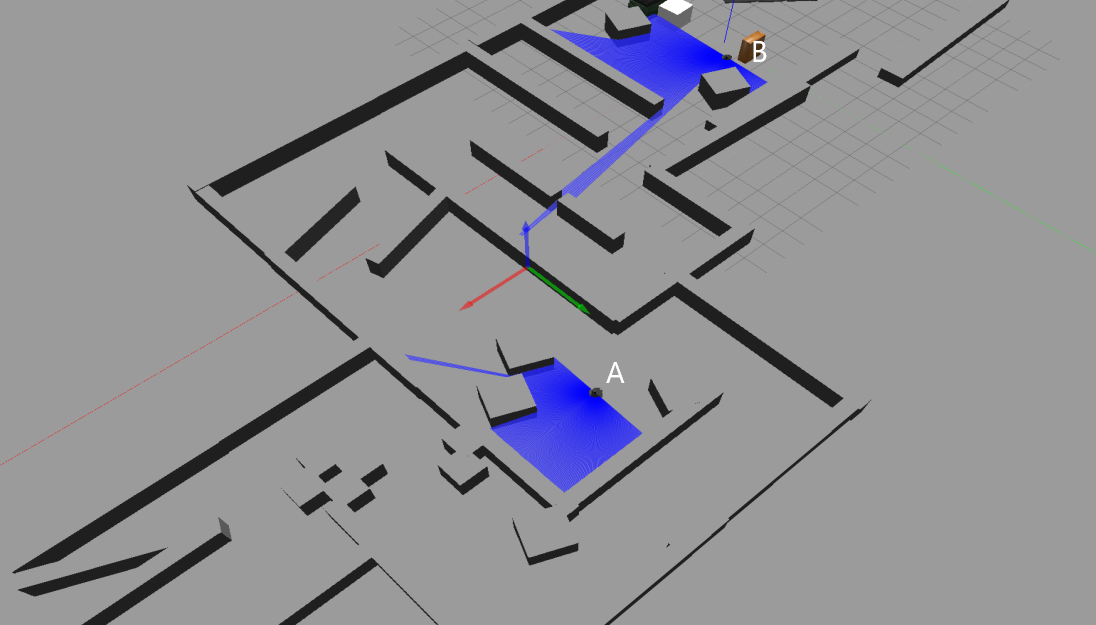
\includegraphics[width=1\textwidth]{figs/gazebo_environment.png}
%----------------------------------------------------
    \caption{Gazebo \(gzclient\) generated from the \(gzserver\). The \(gzserver\) generated the simulation world using a world file and model files. This figure describes two robots (annotated by A and B) and lidar sensor (which are the blue rays are laser rays) in an environment.}
%----------------------------------------------------
    \label{fig:gazebo-environment}
\end{figure}
%....................................................



Figure \ref{fig:maze_arena}, is the layout of the simulation environment used in this experiment. The environment shows two robots simulated in Gazebo building partial maps of the environment, a transform tree diagram with the coordinate frames associated with each robot is presented in Figure \ref{fig:rosgraph-gazebo}, each frame having a prefix to inform ROS which robot it belongs to. The graph also shows the average rate of message exchange transforms and the existing frames of the robots. The simulated robots are Kobuki platforms (see Figure \ref{fig:kuboki-platform-gazebo}) equipped with Hokuyo laser range finders, these robots are selected to match the real-world robot platform used. The simulated Kokoki Platform is controlled using the \(turtlebot\_teleop\)\footnote{http://wiki.ros.org/turtlebot\_teleop} node, through the keyboard. The simulated environment is run on a Windows 10 laptop with the following specifications; Intel Core i5-8250U processor with 16 GB of RAM. The simulated environment is run on a virtual machine using VirtualBox, and the machine can be found on \footnote{googledrive}. The simulated environment is used to initially test the solution proposed in a controlled environment with known parameters. 

%....................................................
\begin{figure}[H]
%----------------------------------------------------
    \centering
%----------------------------------------------------
    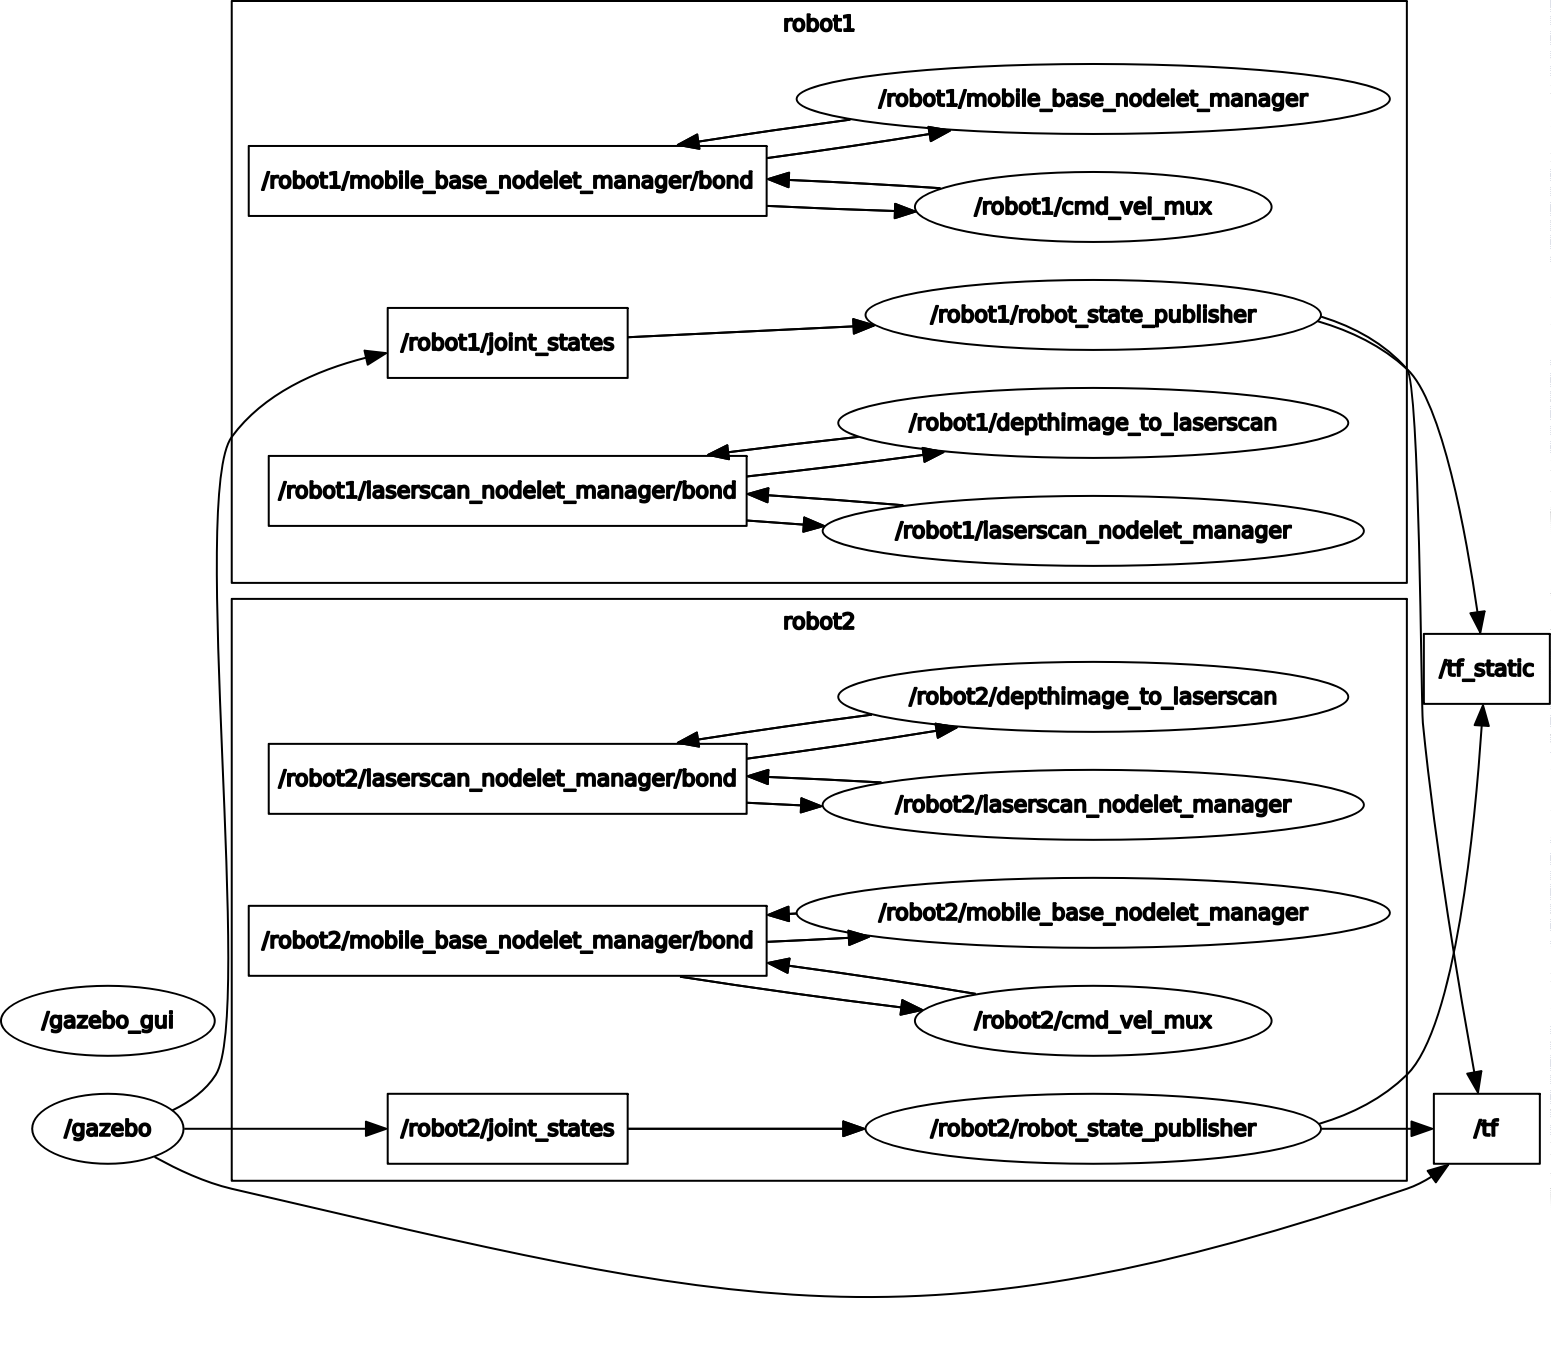
\includegraphics[width=0.9\textwidth]{figs/rosgraph.png}
%----------------------------------------------------
    \caption{ROS graph for simulation environment shown in Figure \ref{fig:gazebo-environment}.}
%----------------------------------------------------
    \label{fig:rosgraph-gazebo}
%----------------------------------------------------
\end{figure}
%....................................................


%....................................................
\begin{figure}[H]
    \centering
    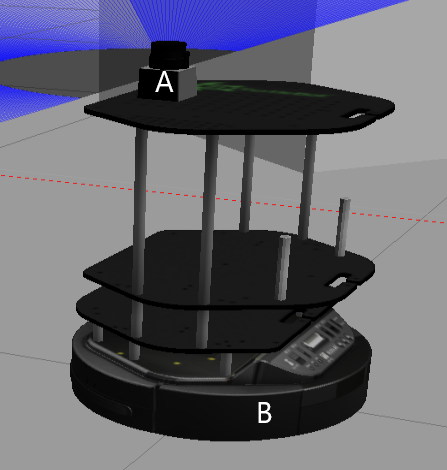
\includegraphics[width=0.5\textwidth]{figs/Kuboki_Platform_Gazebo.png}
    \caption{Kobuki Platform (annotated by (B)) in Gazebo environment. The Platform has a Hokuyo UTM-30LX (annotated by (A) also simulated. Note that the laser rays (blue lines) were limited to 180 degrees. This is all simulated using Gazebo.}
    \label{fig:kuboki-platform-gazebo}
\end{figure}
%....................................................

%....................................................
\begin{figure}[H]
    \centering
    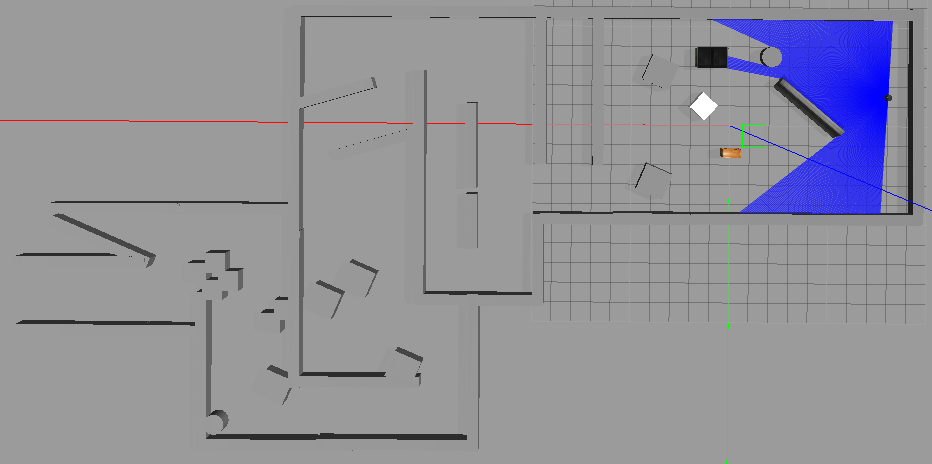
\includegraphics[width=1\textwidth]{figs/maze_area.png}
    \caption{Gazebo simulation environment, with obstacle around the map. There is a Kobuki Platform, with a Hokuyo UTM-30LX attached to it, these are also simulated. }
    \label{fig:maze_arena}
\end{figure}
%....................................................

%====================================================
\subsection{Results and discussion}
\label{sec:sim_results}
%----------------------------------------------------
In this section, simulation results using Gazebo and ROS are presented. 

%==================================================== 
\subsubsection{Experiment one} %----------------------------------------------------

Figures \ref{fig:sim11} and \ref{fig:sim12} represent each robot's partial local map before the merging operation. The local partial maps have a resolution of 0.1 m/cell. Figure \ref{fig:sim13} presents the global map with a resolution of 0.1 m/cell, after merging the partial maps. The global map shows that the partial maps were adequately aligned and merged. The new resolution of partial\_map\_2 is within 1\% of partial\_map\_1's resolution (shown in Table \ref{table:sim1}), therefore validating the success of the alignment operation.  

%....................................................
\begin{figure}[H]
%----------------------------------------------------
\begin{subfigure}{0.5\textwidth}
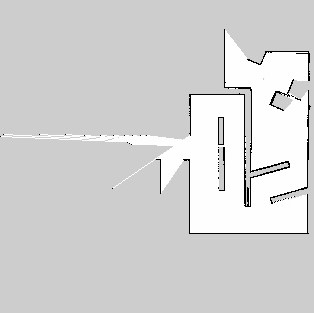
\includegraphics[width=0.9\linewidth, height=5cm]{figs/simulation_results/a/partial_map_1.jpg} 
\caption{Partial map\_1 with resolution of 0.1 m/cell}
\label{fig:sim11}
\end{subfigure}
%----------------------------------------------------
\begin{subfigure}{0.5\textwidth}
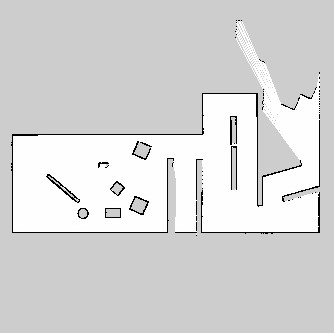
\includegraphics[width=0.9\linewidth, height=5cm]{figs/simulation_results/a/partial_map_2.jpg} 
\caption{Partial map\_2 with resolution of 0.1 m/cell}
\label{fig:sim12}
\end{subfigure}
%----------------------------------------------------
\begin{subfigure}{0.5\textwidth}
\centering
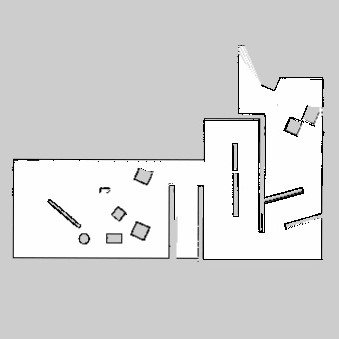
\includegraphics[width=0.9\linewidth, height=5cm]{figs/simulation_results/a/final_map.jpg} 
\caption{Global map with resolution of 0.1 m/cell}
\label{fig:sim13}
\end{subfigure}
%----------------------------------------------------
\caption{Partial maps and a global map are presented. The partial maps are generated from simulated data. Since the maps are aligned relative to map\_1, the resultant global map will have the same resolution as partial map\_1.}
\label{fig:sim1}
\end{figure}
%....................................................

Figure \ref{fig:sim1match1} presents the matched features in the partial maps' overlapping area. There are 30 matched features with a match ratio of 0.46, where the percentage of overlapping area is 35.36\% (see Table \ref{table:sim1}). The match ratio value is influenced by the fact that partial\_map\_2 has most of its features within the overlapping area.


%....................................................
\begin{figure}[H]
    \centering
    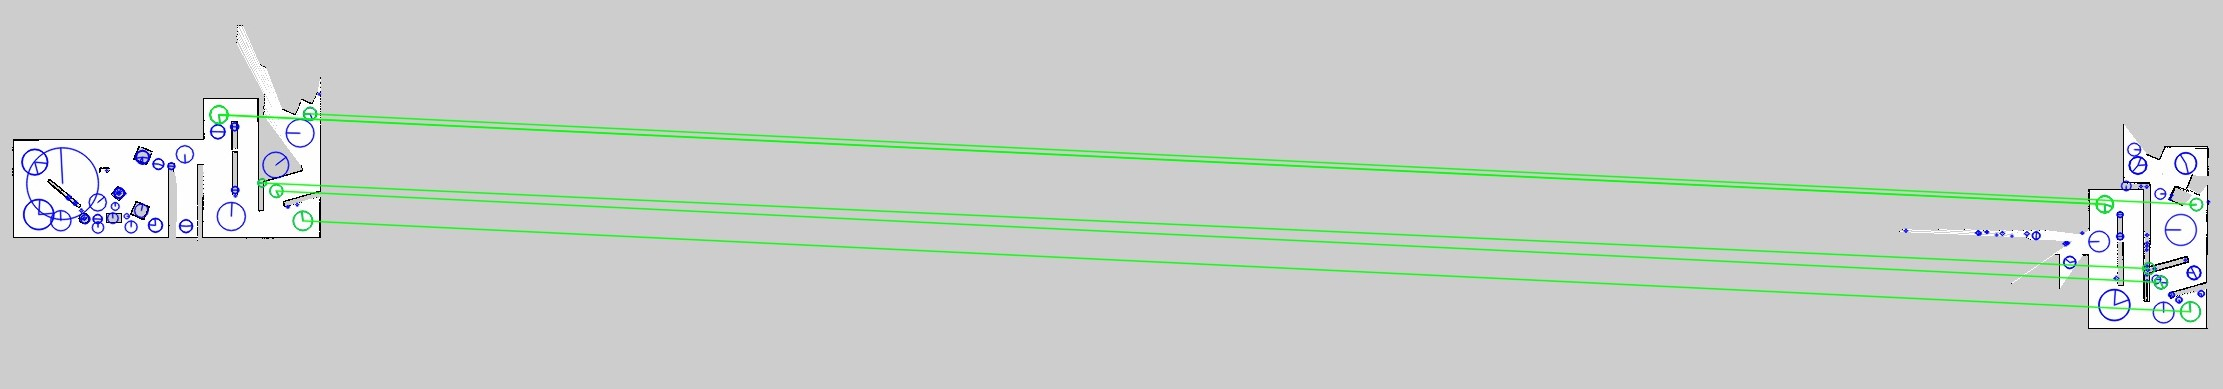
\includegraphics[width=1\textwidth]{figs/simulation_results/a/matchesPartialMap1Map2.jpg}
    \caption{The matched features between partial map\_1 and map\_2 are presented in this figure. The features highlighted in green, are the features that have been matched between the two maps.}
    \label{fig:sim1match1}
\end{figure} 
%....................................................

%....................................................
\begin{table}[H]
\centering
\caption{This table presents the results from the alignment and merging operation. Since the partial maps are merged relatively to map\_1, the results are relative to map\_1, which has a resolution of 0.1 m/cell.}

%----------------------------------------------------
\begin{tabular}{ | m{1.4cm} | m{2.2cm} | m{2.2cm} | m{2.4cm} | m{1.7cm} | m{1.4cm} | m{2.4cm} | } 
\hline
\textbf{Map} & \textbf{Resolution (m/cell)} & \textbf{New resolution (m/cell)} & \textbf{Angle of rotation (\degree)} & \textbf{Good matches} & \textbf{Match ratio} & \textbf{Percentage overlap}\\ 
\hline 
\hline
Partial map\_2  & 0.1  & 0.09956828 & -0.16716242 & 30 & 0.46 & 35.36 \\ 
\hline
\end{tabular}
%----------------------------------------------------
\label{table:sim1}
\end{table}
%....................................................

%==================================================== 
\subsubsection{Experiment two} 
%----------------------------------------------------

The next results still consider two robots with the same resolution partial\_maps, but the maps have a bigger overlapping area of 48.03\% (see Table \ref{table:sim2}). Figures \ref{fig:sim21} and \ref{fig:sim22} represent each robot's partial local map before the merging operation. The local partial maps have a resolution of 0.1 m/cell. Figure\ref{fig:sim13} presents the global map of 0.1 m/cell, after the merging of the partial maps. The global map shows that the partial maps were adequately aligned and merged. The new resolution of partial\_map\_2 is within 1\% of partial\_map\_1's resolution (shown in Table \ref{table:sim2}), therefore validating the success of the alignment operation.  

%....................................................
\begin{figure}[H]
%----------------------------------------------------
\begin{subfigure}{0.5\textwidth}
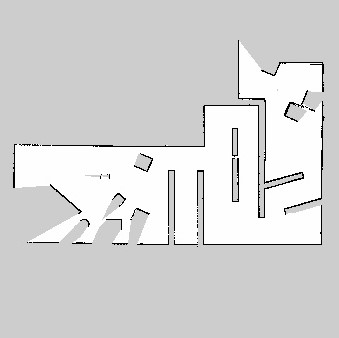
\includegraphics[width=0.9\linewidth, height=5cm]{figs/simulation_results/b/partial_map_1.jpg} 
\caption{Partial map\_1 resolution of 0.1 m/cell}
\label{fig:sim21}
\end{subfigure}
%----------------------------------------------------
\begin{subfigure}{0.5\textwidth}
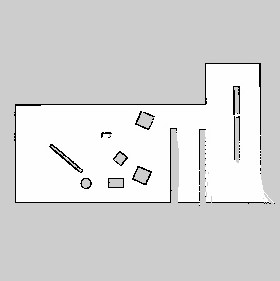
\includegraphics[width=0.9\linewidth, height=5cm]{figs/simulation_results/b/partial_map_2.jpg} 
\caption{Partial map\_2 resolution of 0.1 m/cell}
\label{fig:sim22}
\end{subfigure}
%----------------------------------------------------
\begin{subfigure}{0.5\textwidth}
\centering
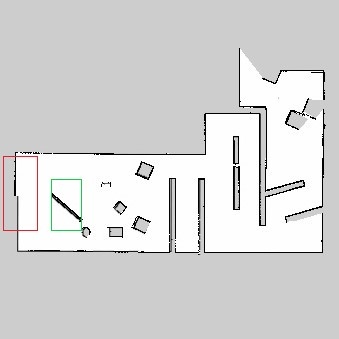
\includegraphics[width=0.9\linewidth, height=5cm]{figs/simulation_results/b/final_map_marked.jpg}
\caption{Global map of resolution of 0.1 m/cell}
\label{fig:sim23}
\end{subfigure}
%----------------------------------------------------
\caption{Partial maps and a global map are presented. The partial maps are generated from simulated data. Since the maps are aligned relative to map\_1, the resultant global map will have the same resolution as partial map\_1.}
\label{fig:sim2}
\end{figure}
%....................................................


Unlike results Figure \ref{fig:sim1}, Figure \ref{fig:sim2} a slight misalignment which is highlighted in red and green. Figure \ref{fig:sim2match1} shows that the features in the green and red area were not matched, therefore causing the misalignment. Despite the fact that the match ratio and percentage overlap of 0.59 and 48\%, are higher here (see Table \ref{table:sim2}) than in the previous ((see Table \ref{table:sim1}) results. This result suggests that it is important that the matches are evenly distributed throughout the overlapping region with a high match ratio. 

%....................................................
\begin{figure}[H]
    \centering
    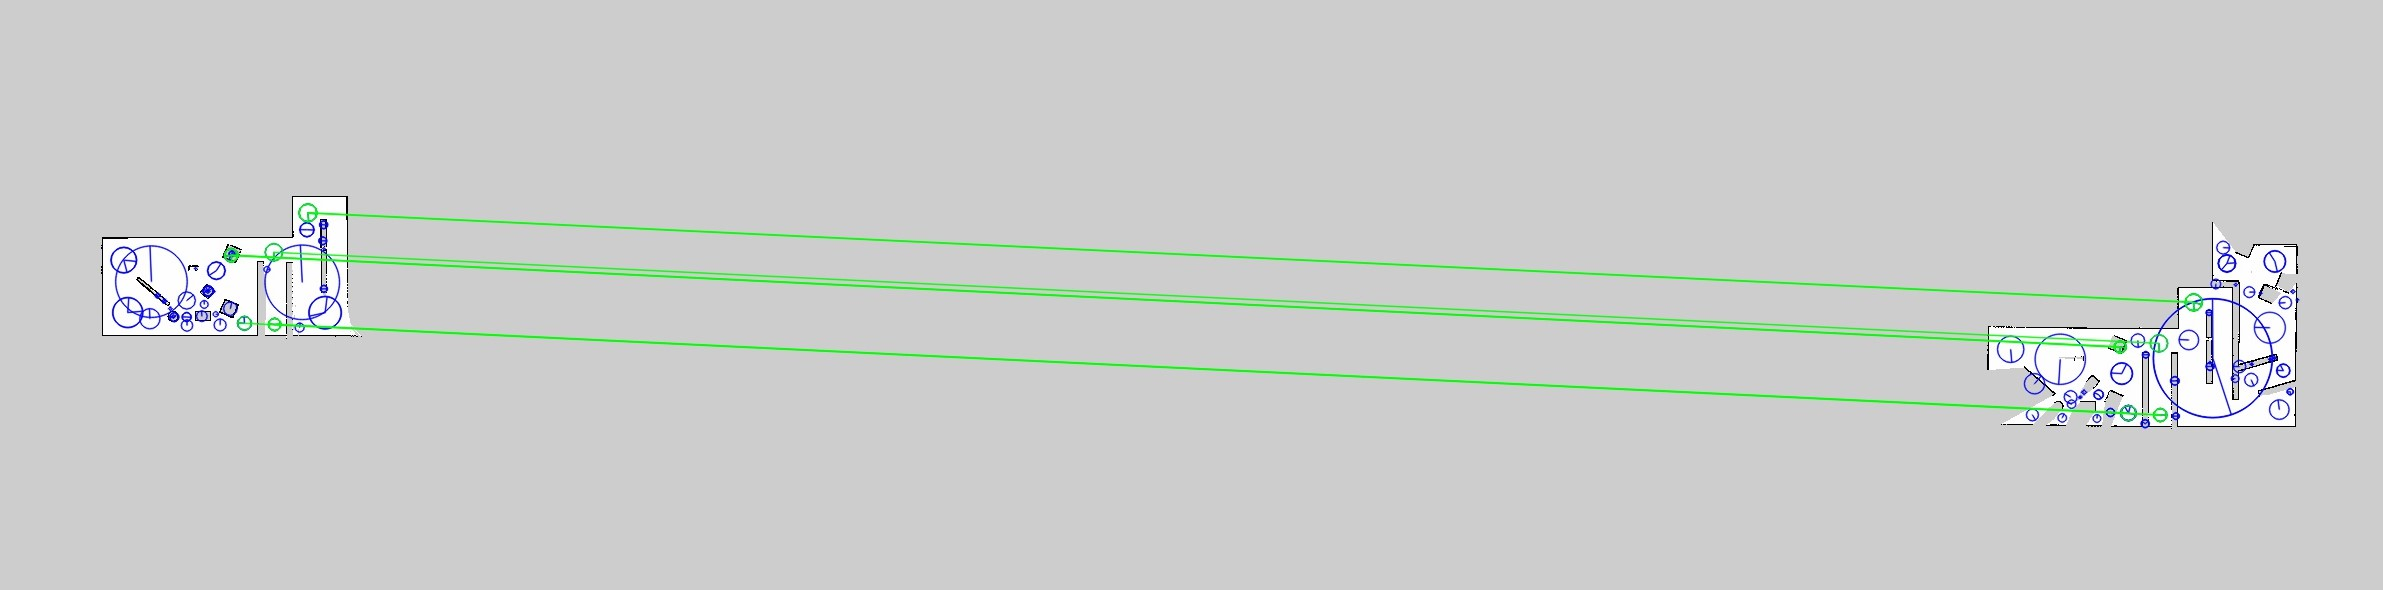
\includegraphics[width=1\textwidth]{figs/simulation_results/b/matchesPartialMap1Map2.jpg}
    \caption{The matched features between partial map\_1 and map\_2 are presented in this figure. The features highlighted in green, are the features that have been matched between the two maps.}
    \label{fig:sim2match1}
\end{figure} 
%....................................................



%....................................................
\begin{table}[H]
\centering
\caption{This table presents the results from the alignment and merging operation. Since the partial maps are merged relatively to map\_1 the results are relative to map\_1, which  has a resolution of 0.1 m/cell.}
\begin{tabular}{ | m{1.4cm} | m{2.2cm} | m{2.2cm} | m{2.4cm} | m{1.7cm} | m{1.4cm} | m{2.4cm} | }
\hline
\textbf{Map} & \textbf{Resolution (m/cell)} & \textbf{New resolution (m/cell)} & \textbf{Angle of rotation (\degree)} & \textbf{Good matches} & \textbf{Match ratio} & \textbf{Percentage overlap}\\ 
\hline
\hline
Partial map\_2  & 0.1  & 0.10111790 & -0.08469242 & 36 & 0.59 & 48.03\\ 
\hline
\end{tabular}
\label{table:sim2}
\end{table}
%....................................................

%==================================================== 
\subsubsection{Experiment three} %----------------------------------------------------

Figures \ref{fig:sim31}, \ref{fig:sim32} and \ref{fig:sim33} represent partial maps from three robots before the merging operation. The local partial maps have a resolution of 0.1 m/cell. The maps are to be transformed into partial\_map\_1's frame of reference. Figure \ref{fig:sim34} presents the global map of 0.1 m/cell, after merging the partial maps. The global map shows that the partial map\_2 and map\_3 were adequately aligned into map\_1 and merged. The new resolution of partial\_map\_2 and partial\_map\_3 are both within 1\% of partial\_map\_1's resolution (shown in Table \ref{table:sim3}) validating the success of the alignment operation.  

%....................................................
\begin{figure}[H]
\begin{subfigure}{0.5\textwidth}
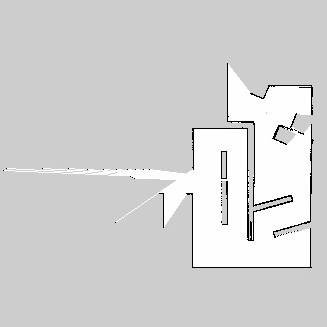
\includegraphics[width=0.9\linewidth, height=5cm]{figs/simulation_results/c/partial_map_1.jpg} 
\caption{Partial map\_1 with resolution of 0.1 m/cell}
\label{fig:sim31}
\end{subfigure}
\begin{subfigure}{0.5\textwidth}
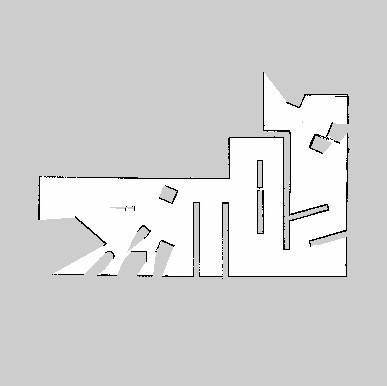
\includegraphics[width=0.9\linewidth, height=5cm]{figs/simulation_results/c/partial_map_2.jpg} 
\caption{Partial map\_2 with resolution of 0.1 m/cell}
\label{fig:sim32}
\end{subfigure}
\begin{subfigure}{0.5\textwidth}
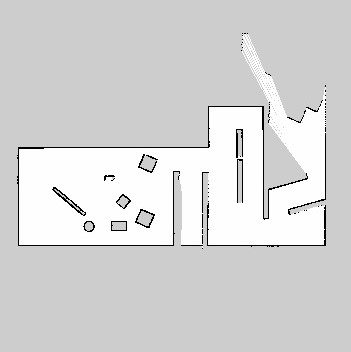
\includegraphics[width=0.9\linewidth, height=5cm]{figs/simulation_results/c/partial_map_3.jpg} 
\caption{Partial map\_2 with resolution of 0.1 m/cell}
\label{fig:sim33}
\end{subfigure}
\begin{subfigure}{0.5\textwidth}
\centering
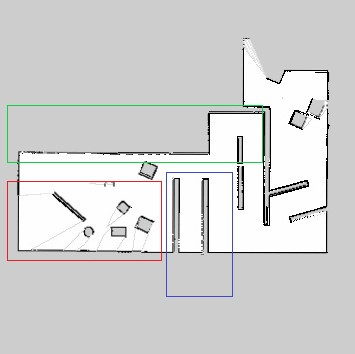
\includegraphics[width=0.9\linewidth, height=5cm]{figs/simulation_results/c/final_map_marked.jpg} 
\caption{Global map with resolution of 0.1 m/cell}
\label{fig:sim34}
\end{subfigure}
\caption{Three partial maps and a global map are presented. The partial maps are generated from simulated data. Since the maps are aligned relative to map\_1, the resultant global map will have the same resolution as partial map\_1.}
\label{fig:sim3}
\end{figure}
%....................................................


Given that the matches are mostly on the rightmost position (see figures \ref{fig:sim3match1} and  \ref{fig:sim3match2}) due to partial map\_1, results similar to Figure \ref{fig:sim2} are expected. The red regions in Figure \ref{fig:sim34} have unknown(grey) regions, likely because map\_2 and map\_3 are unaware of each other. However, the blue and green region in Figure \ref{fig:sim34} shows information from map\_2 and map\_3 being successfully included in the global\_map. 

Table \ref{table:sim3} shows match ratio results and percentage overlap, suggesting that a higher percentage produces a higher match ratio. This relationship will be evaluated in the next experiments too.

%....................................................
\begin{figure}[H]
    \centering
    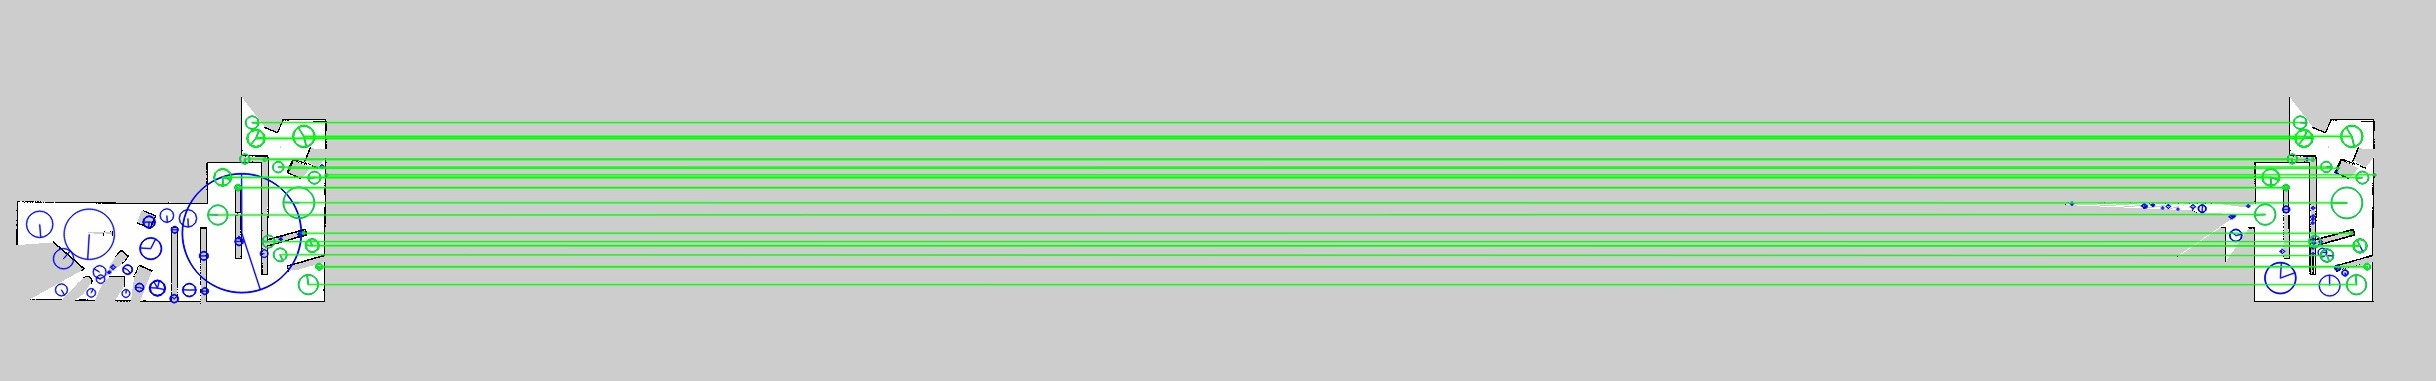
\includegraphics[width=1\textwidth]{figs/simulation_results/c/matchesPartialMap1Map2.jpg}
    \caption{The matched features between partial map\_1 and map\_2 are presented in this figure. The features highlighted in green, are the features that have been matched between the two maps.}
    \label{fig:sim3match1}
\end{figure} 
%....................................................

%....................................................
\begin{figure}[H]
    \centering
    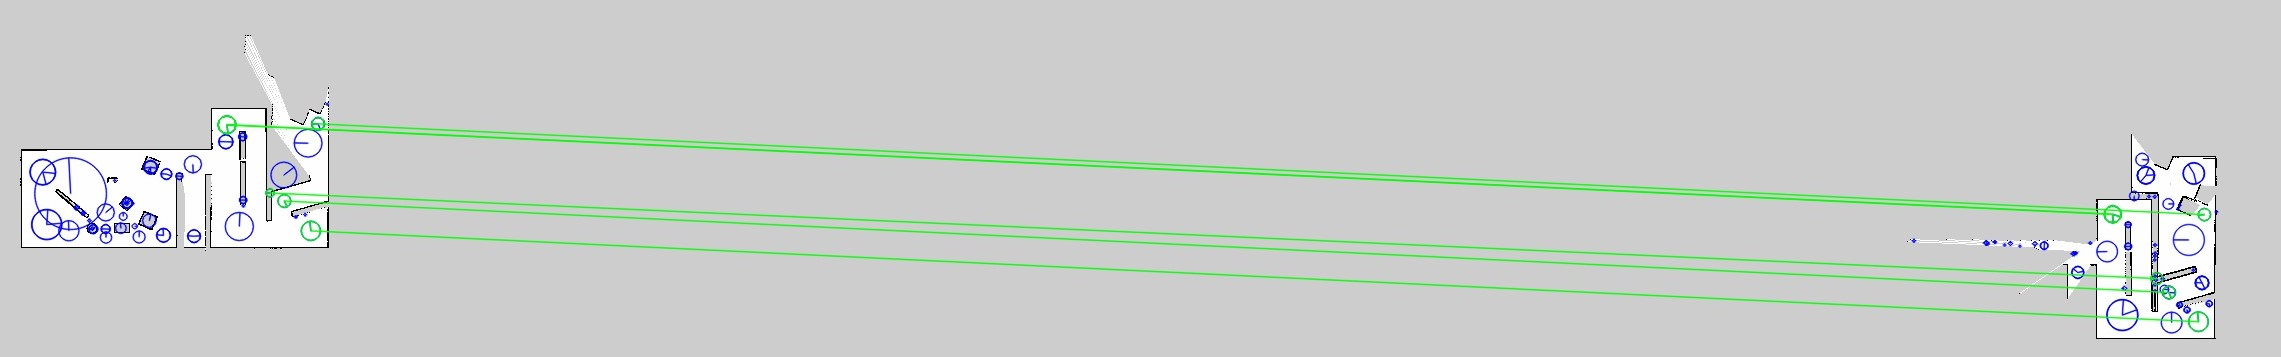
\includegraphics[width=1\textwidth]{figs/simulation_results/c/matchesPartialMap1Map3.jpg}
    \caption{The matched features between partial map\_1 and map\_3 are presented in this figure. The features highlighted in green, are the features that have been matched between the two maps.}
    \label{fig:sim3match2}
\end{figure} 
%....................................................

%....................................................
\begin{table}[H]
\centering
\caption{This table presents the results from the alignment and merging operation. Since the partial maps are merged relatively to map\_1 the results are relative to map\_1, which  has a resolution of 0.1 m/cell.}

\begin{tabular}{ | m{1.4cm} | m{2.2cm} | m{2.2cm} | m{2.4cm} | m{1.7cm} | m{1.4cm} | m{2.4cm} | } 
\hline
\textbf{Map} & \textbf{Resolution (m/cell)} & \textbf{New resolution (m/cell)} & \textbf{Angle of rotation (\degree)} & \textbf{Good matches} & \textbf{Match ratio} & \textbf{Percentage Overlap}\\ 
\hline
\hline
Partial map\_2  & 0.1  & 0.09985444 & -0.13717321 & 40 & 0.56 & 50.83502376\\ 
\hline
Partial map\_3  & 0.1  & 0.09956828 & -0.16716242 & 30 & 0.46 & 35.36\\ 
\hline
\end{tabular}
\label{table:sim3}
\end{table}
%....................................................


%==================================================== 
\subsubsection{Experiment four} 
%----------------------------------------------------

Figures \ref{fig:sim41} and \ref{fig:sim42} represents the partial maps of two robots at different resolutions (0.2 m/cell and 0.1 m/cell) before the alignment and merging operation. Partial\_map\_1 in Figure \ref{fig:sim41}, presents a mapping error highlighted in yellow, compared with original arena in Figure \ref{fig:maze_arena}. The mapping error has caused the map in the yellow region to rotate slightly. Despite the error a global map was successfully produced (see Figure \ref{fig:sim43}). These merging defects can be seen mostly in the red and green regions of the global\_map(Figure \ref{fig:sim43}); however the defects the information of partial\_map 2 have successfully been included in the map. The new resolution of partial\_map\_2 is with in 1\% of partial\_map\_1, which further validates the success of the merge (see Table \ref{table:sim4}).


%....................................................
\begin{figure}[H]
\begin{subfigure}{0.5\textwidth}
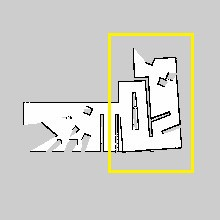
\includegraphics[width=0.9\linewidth, height=5cm]{figs/simulation_results/c_diff_resolution/partial_map_1_marked.jpg} 
\caption{Partial map\_1 with resolution of 0.2 m/cell}
\label{fig:sim41}
\end{subfigure}
\begin{subfigure}{0.5\textwidth}
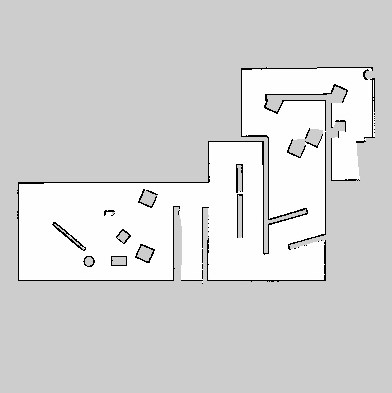
\includegraphics[width=0.9\linewidth, height=5cm]{figs/simulation_results/c_diff_resolution/partial_map_2.jpg} 
\caption{Partial map\_2 with resolution of 0.1 m/cell}
\label{fig:sim42}
\end{subfigure}
\begin{subfigure}{0.5\textwidth}
\centering
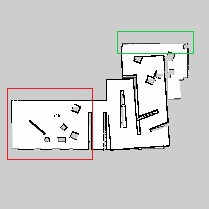
\includegraphics[width=0.9\linewidth, height=5cm]{figs/simulation_results/c_diff_resolution/final_map_marked.jpg} 
\caption{Global map with resolution of 0.2 m/cell}
\label{fig:sim43} 
\end{subfigure}
\caption{Two partial maps and a global map are presented. The partial maps are generated from simulated data, and they are of varying resolution. Since the maps are aligned relative to map\_1, the resultant global map will have the same resolution as partial map\_1.}
\label{fig:sim4}
\end{figure}
%....................................................


Figure \ref{fig:sim4match1} represents the matches between partial\_maps 1 and 2, with a match ratio of 0.66 and percentage overlap of 52.93\% (see Table \ref{table:sim4}). Again there is evidence of a directly proportional relationship between percentage overlap and match ratio compared to the previous experiment.


%....................................................
\begin{figure}[H]
    \centering
    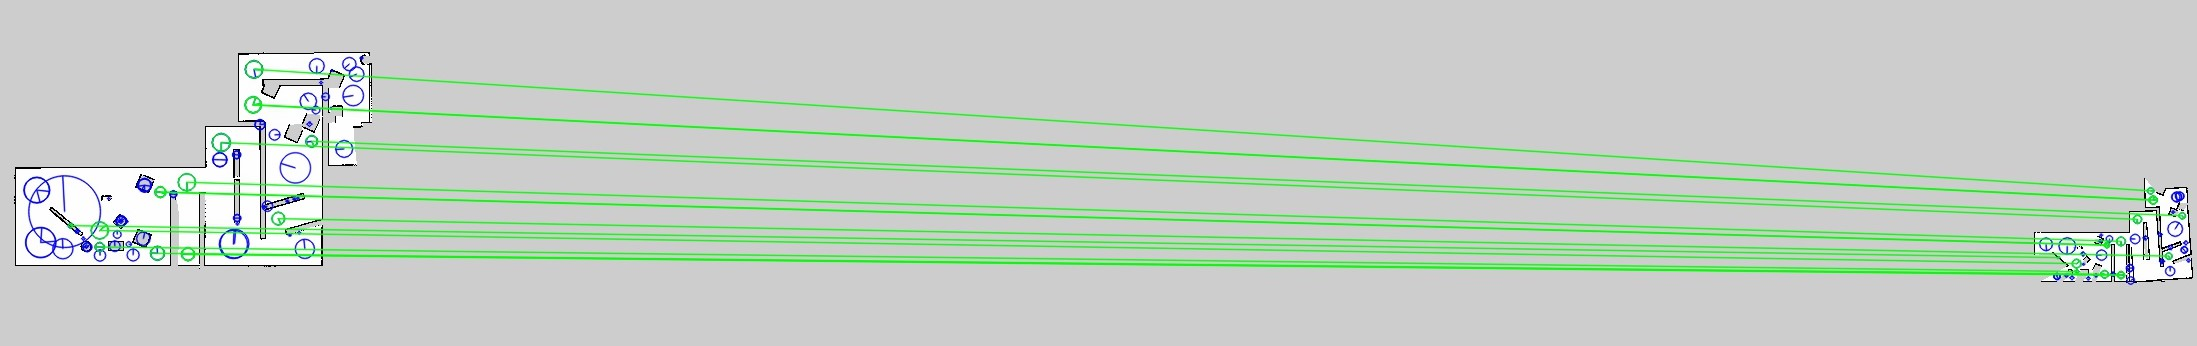
\includegraphics[width=1\textwidth]{figs/simulation_results/c_diff_resolution/matchesPartialMap1Map2.jpg}
     \caption{The matched features between partial map\_1 and map\_2 are presented in this figure. The features highlighted in green, are the features that have been matched between the two maps.}
    \label{fig:sim4match1}
\end{figure} 
%....................................................

%....................................................
\begin{table}[H]
\centering
\caption{This table presents the results from the alignment and merging operation. Since the partial maps are merged relatively to map\_1 the results are relative to map\_1, which  has a resolution of 0.2 m/cell.}
\begin{tabular}{ | m{1.4cm} | m{2.2cm} | m{2.2cm} | m{2.4cm} | m{1.7cm} | m{1.4cm} | m{2.4cm} | }
\hline
\textbf{Map} & \textbf{Resolution (m/cell)} & \textbf{New resolution (m/cell)} & \textbf{Angle of rotation (\degree)} & \textbf{Good matches} & \textbf{Match ratio} & \textbf{Percentage overlap}\\ 
\hline
\hline
Partial map\_2  & 0.1  & 0.20177466 & 0.03968788 & 35 & 0.66 & 52.93\\ 
\hline
\end{tabular}
\label{table:sim4}
\end{table}
%....................................................

%==================================================== 
\subsubsection{Experiment five} %----------------------------------------------------

The final simulation experiment presents three partial maps aligned and merged to form a global map (see Figure \ref{fig:sim5}). Partial map\_2 and map\_3 have a resolution of 0.1 m/cell, which is different from map\_1's resolution of 0.2 m/cell. The global map in Figure \ref{fig:sim54}, is a result of the alignment and merging of maps 2 and 3 into map\_1's reference frame. Similarly to Figure \ref{fig:sim41}, Figure \ref{fig:sim51} has a mapping error, which has been incorporated into the global map. However, the errors both map\_2 and map\_3's new resolutions are within 1\% of map\_1's resolutions. 


%....................................................
\begin{figure}[H]
\begin{subfigure}{0.5\textwidth}
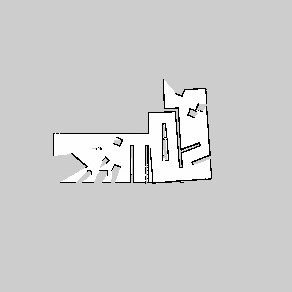
\includegraphics[width=0.9\linewidth, height=5cm]{figs/simulation_results/d_diff_resolution/partial_map_1.jpg} 
\caption{Partial map\_1 with resolution of 0.2 m/cell}
\label{fig:sim51}
\end{subfigure}
\begin{subfigure}{0.5\textwidth}
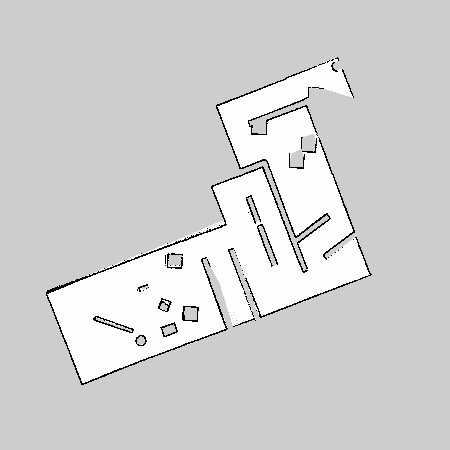
\includegraphics[width=0.9\linewidth, height=5cm]{figs/simulation_results/d_diff_resolution/partial_map_2.jpg} 
\caption{Partial map\_2 with resolution of 0.1 m/cell}
\label{fig:sim52}
\end{subfigure}
\begin{subfigure}{0.5\textwidth}
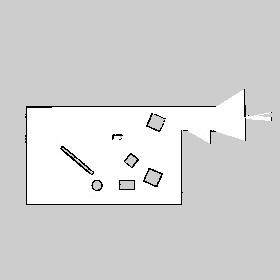
\includegraphics[width=0.9\linewidth, height=5cm]{figs/simulation_results/d_diff_resolution/partial_map_3.jpg} 
\caption{Partial map\_3 with resolution of 0.1 m/cell}
\label{fig:sim53}
\end{subfigure}
\begin{subfigure}{0.5\textwidth}
\centering
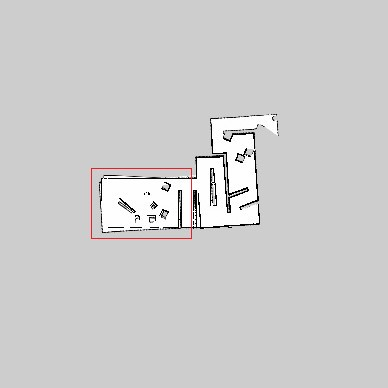
\includegraphics[width=0.9\linewidth, height=5cm]{figs/simulation_results/d_diff_resolution/final_map_marked.jpg} 
\caption{Global map with resolution of 0.2 m/cell}
\label{fig:sim54}
\end{subfigure}
\caption{Three partial maps and a global map are presented. The partial maps are generated from simulated data, and they are of varying resolutions. Since the maps are aligned relative to map\_1, the resultant global map will have the same resolution as partial map\_1.}
\label{fig:sim5}
\end{figure}
%....................................................

Figure \ref{fig:sim5match1} show feature matches between map\_1 and map\_2, with match ratio and percentage overlap of 0.68 and 54.43 respectively (see Table \ref{table:sim5}). Figure \ref{fig:sim5match1} shows feature matches between map\_1 and map\_3, with match ratio and percentage overlap of 0.52 and 27.62 respectively (see Table \ref{table:sim5}). This result again confirms the proportional relationship between the match ratio and percentage overlap.


%....................................................
\begin{figure}[H]
    \centering
    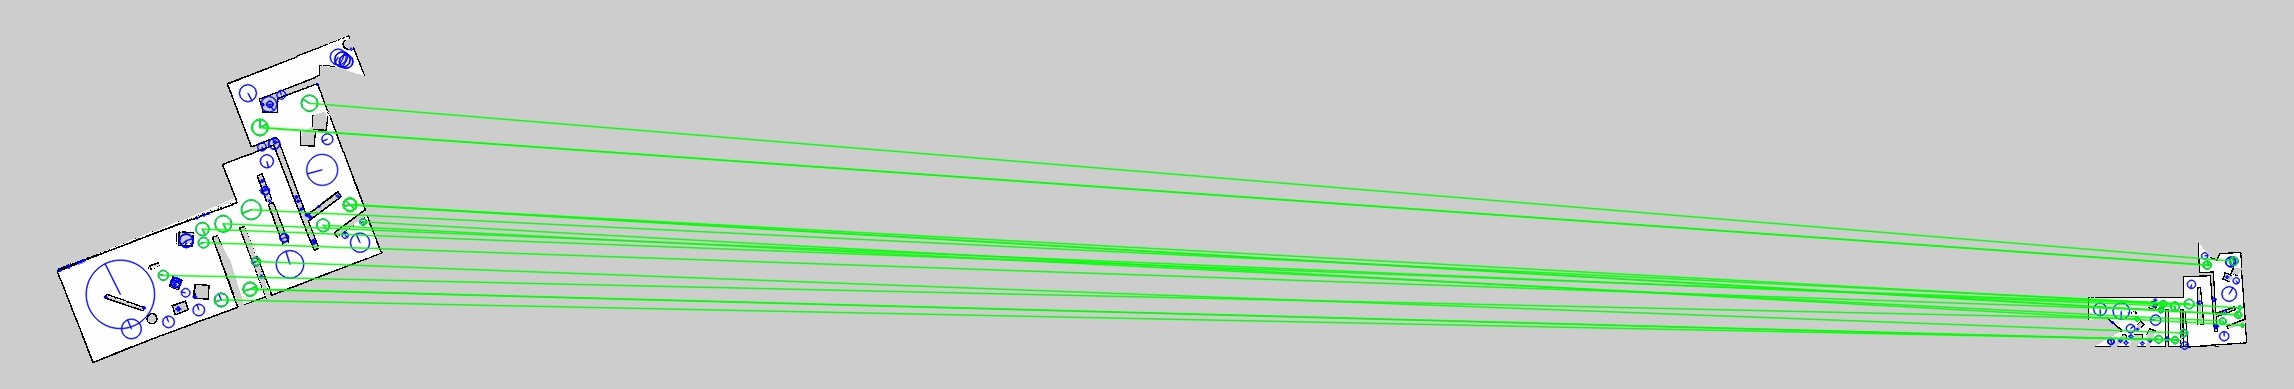
\includegraphics[width=1\textwidth]{figs/simulation_results/d_diff_resolution/matchesPartialMap1Map2.jpg}
    \caption{The matched features between partial map\_1 and map\_2 are presented in this figure. The features highlighted in green, are the features that have been matched between the two maps.}
    \label{fig:sim5match1}
\end{figure} 
%....................................................

%....................................................
\begin{figure}[H]
    \centering
    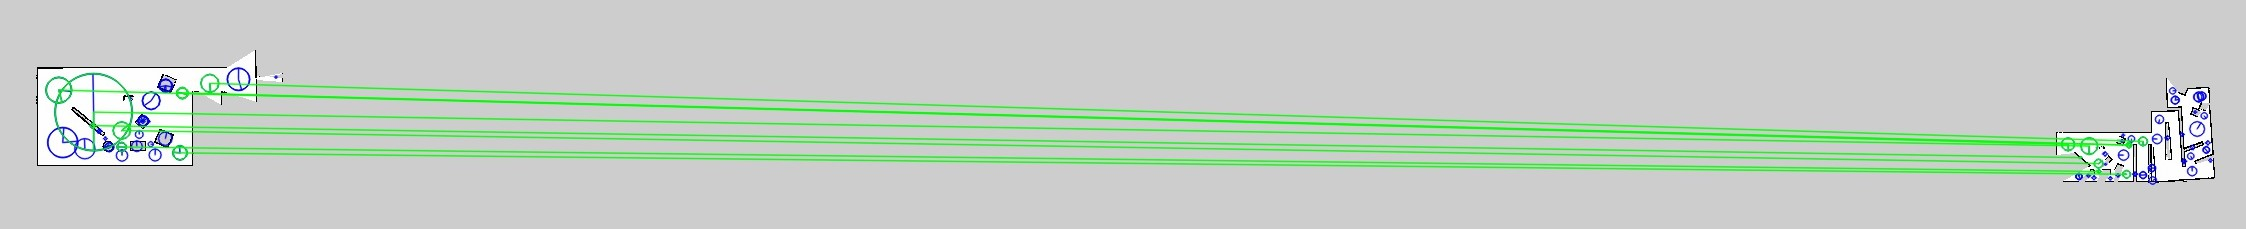
\includegraphics[width=1\textwidth]{figs/simulation_results/d_diff_resolution/matchesPartialMap1Map3.jpg}
    \caption{The matched features between partial map\_1 and map\_3 are presented in this figure. The features highlighted in green, are the features that have been matched between the two maps.}
    \label{fig:sim5match2}
\end{figure} 
%....................................................

%....................................................
\begin{table}[H]
\centering
\caption{This table presents the results from the alignment and merging operation. Since the partial maps are merged relatively to map\_1 the results are relative to map\_1, which  has a resolution of 0.2 m/cell.}
\begin{tabular}{ | m{1.4cm} | m{2.2cm} | m{2.2cm} | m{2.4cm} | m{1.7cm} | m{1.4cm} | m{2.4cm} | }
\hline
\textbf{Map} & \textbf{Resolution (m/cell)} & \textbf{New resolution (m/cell)} & \textbf{Angle of rotation (\degree)} & \textbf{Good matches} & \textbf{Match ratio} & \textbf{Percentage overlap}\\ 
\hline
\hline
Partial map\_2  & 0.1  & 0.1980208 & -17.8182736 & 36 & 0.68 & 54.43\\ 
\hline
Partial map\_3  & 0.1  & 0.2019860 & -2.91611928 & 24 & 0.52 & 27.62\\ 
\hline
\end{tabular}
\label{table:sim5}
\end{table}
%....................................................

\subsubsection{Summary}
The results in this section show that up-to three partial maps with different translations, orientations and resolutions can be aligned and merged successfully to form a global map. The results also show that mapping errors are propagated into the global map. The map merging operation can be limited by the matched feature spread. If matches are concentrated in one area, the merging operation will struggle to match other overlapping areas. We have also observed that the match ratio is directly proportional to the percentage overlap.

Further experiments can now be carried out to test the solution's real-world performance, using this section's results. The next section discusses the experiments carried out in the real world.



%====================================================

\section{Real-world experiments}
\label{subsec:ch4.section1.subsec2}
%----------------------------------------------------

The promising results from the simulation experiments naturally suggested transferring the experiments into the real-world. This section presents a real-world experiment setup and results.

%====================================================
\subsection{Environment setup}
%----------------------------------------------------

The experiments were conducted in the Leslie Social building at the University of Cape Town\footnote{http://www.uct.ac.za/main/contacts/building-list}. This building is a structured indoor environment with minimal natural lighting. Figure \ref{fig:uct_floor} is a floor plan of the fifth floor in the building, and the yellow highlight shows the path travelled by the robot. Using ROS's capability, the robot data is recorded using \(rosbag\)\footnote{http://wiki.ros.org/rosbag}, and later partial maps are generated at a varying resolution for merging.

\begin{figure}[H]
    \centering
    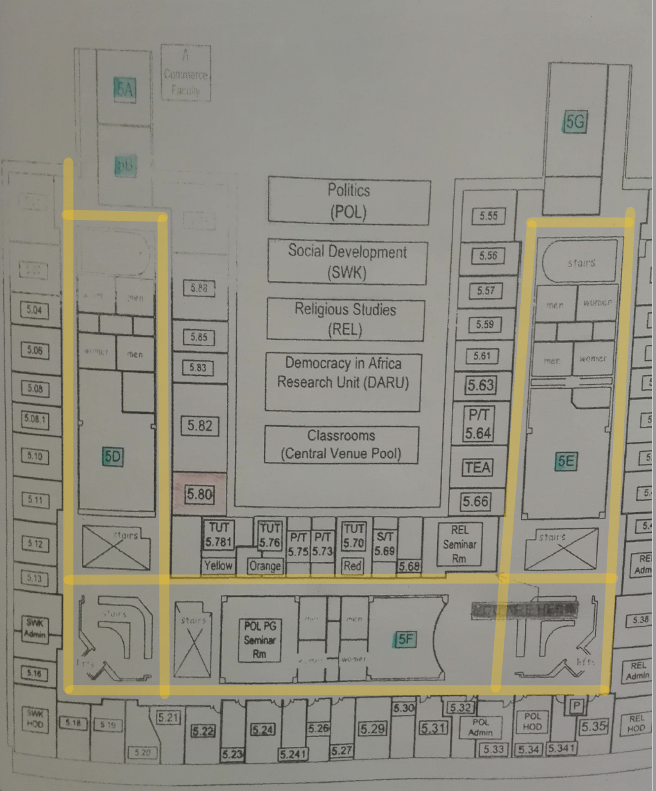
\includegraphics[width=1\textwidth]{figs/real_world_results/original_floor.png}
    \caption{Leslie Social 5th Floor at the University of Cape Town, the yellow shows where the robot moved during the experiment. The partial maps are produced in this area. }
    \label{fig:uct_floor}
\end{figure}


%====================================================
\subsubsection{Kuboki Platform}
%----------------------------------------------------

The chassis shown in Figure \ref{fig:kuboki-platform} is the iClebo Kobuki used in simulation and real-world testing. This platform is a low-cost mobile robot designed for education and research on the state of art robotics. The Kobuki provides power supplies for an external computer and any additional sensors.

%....................................................
\begin{figure}[H]
    \centering
    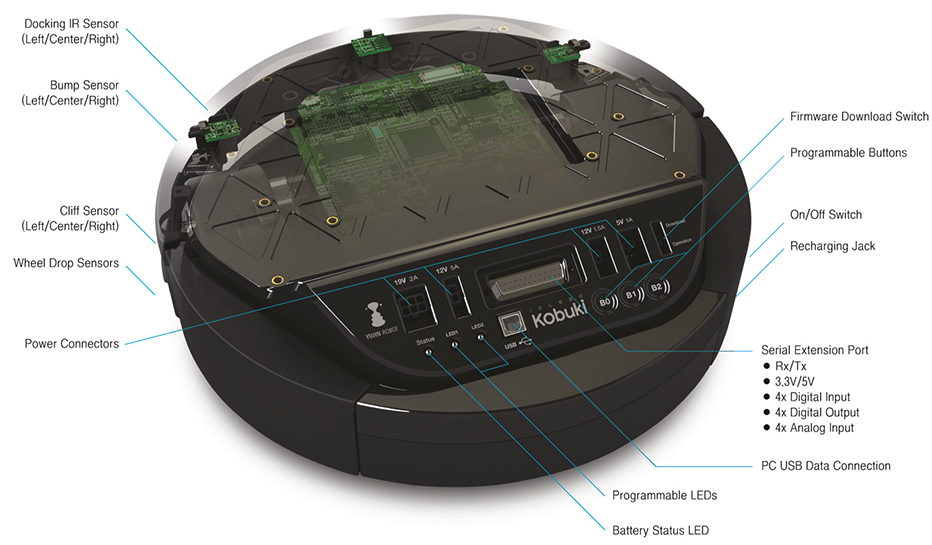
\includegraphics[width=0.9\textwidth]{figs/Kuboki_Platform.png}
    \caption[Kobuki platform]{Kobuki platform without attachments. Taken from \footnote{http://kobuki.yujinrobot.com/about2/}.}
    \label{fig:kuboki-platform} 
\end{figure}
%....................................................

The platform in Figure \ref{fig:turtle_bot_experiments}, is set up with a Hokuyo UTM-30LX and Raspberry Pi 3B with ROS installed. The Kobuki platform can travel at a maximum of 70 cm/s translational velocity, and a maximum rotational velocity of 180 \degree/s, however above 110 \degree/s performance will degrade. The platform can take a maximum payload of 5 kg. The platform has safety measures to ensure safe usage, and these include a cliff detector (to avoid driving off cliffs of a depth greater than 5cm) and a climbing threshold (to avoid climbing elevations above 12 mm). The expected operating time is 3/7hours (small/large battery), and the expected charging time is 1.5/2.6 hours (small/large battery). 

The Kobuki platform can be controlled using the Robot Operating System (ROS), a repository is provided on \footnote{https://github.com/yujinrobot/kobuki}. This repository also offers simulation models that can be used to simulate the platform in Gazebo or \textit{stage\_ros}.


 \begin{figure}[H]
    \centering
    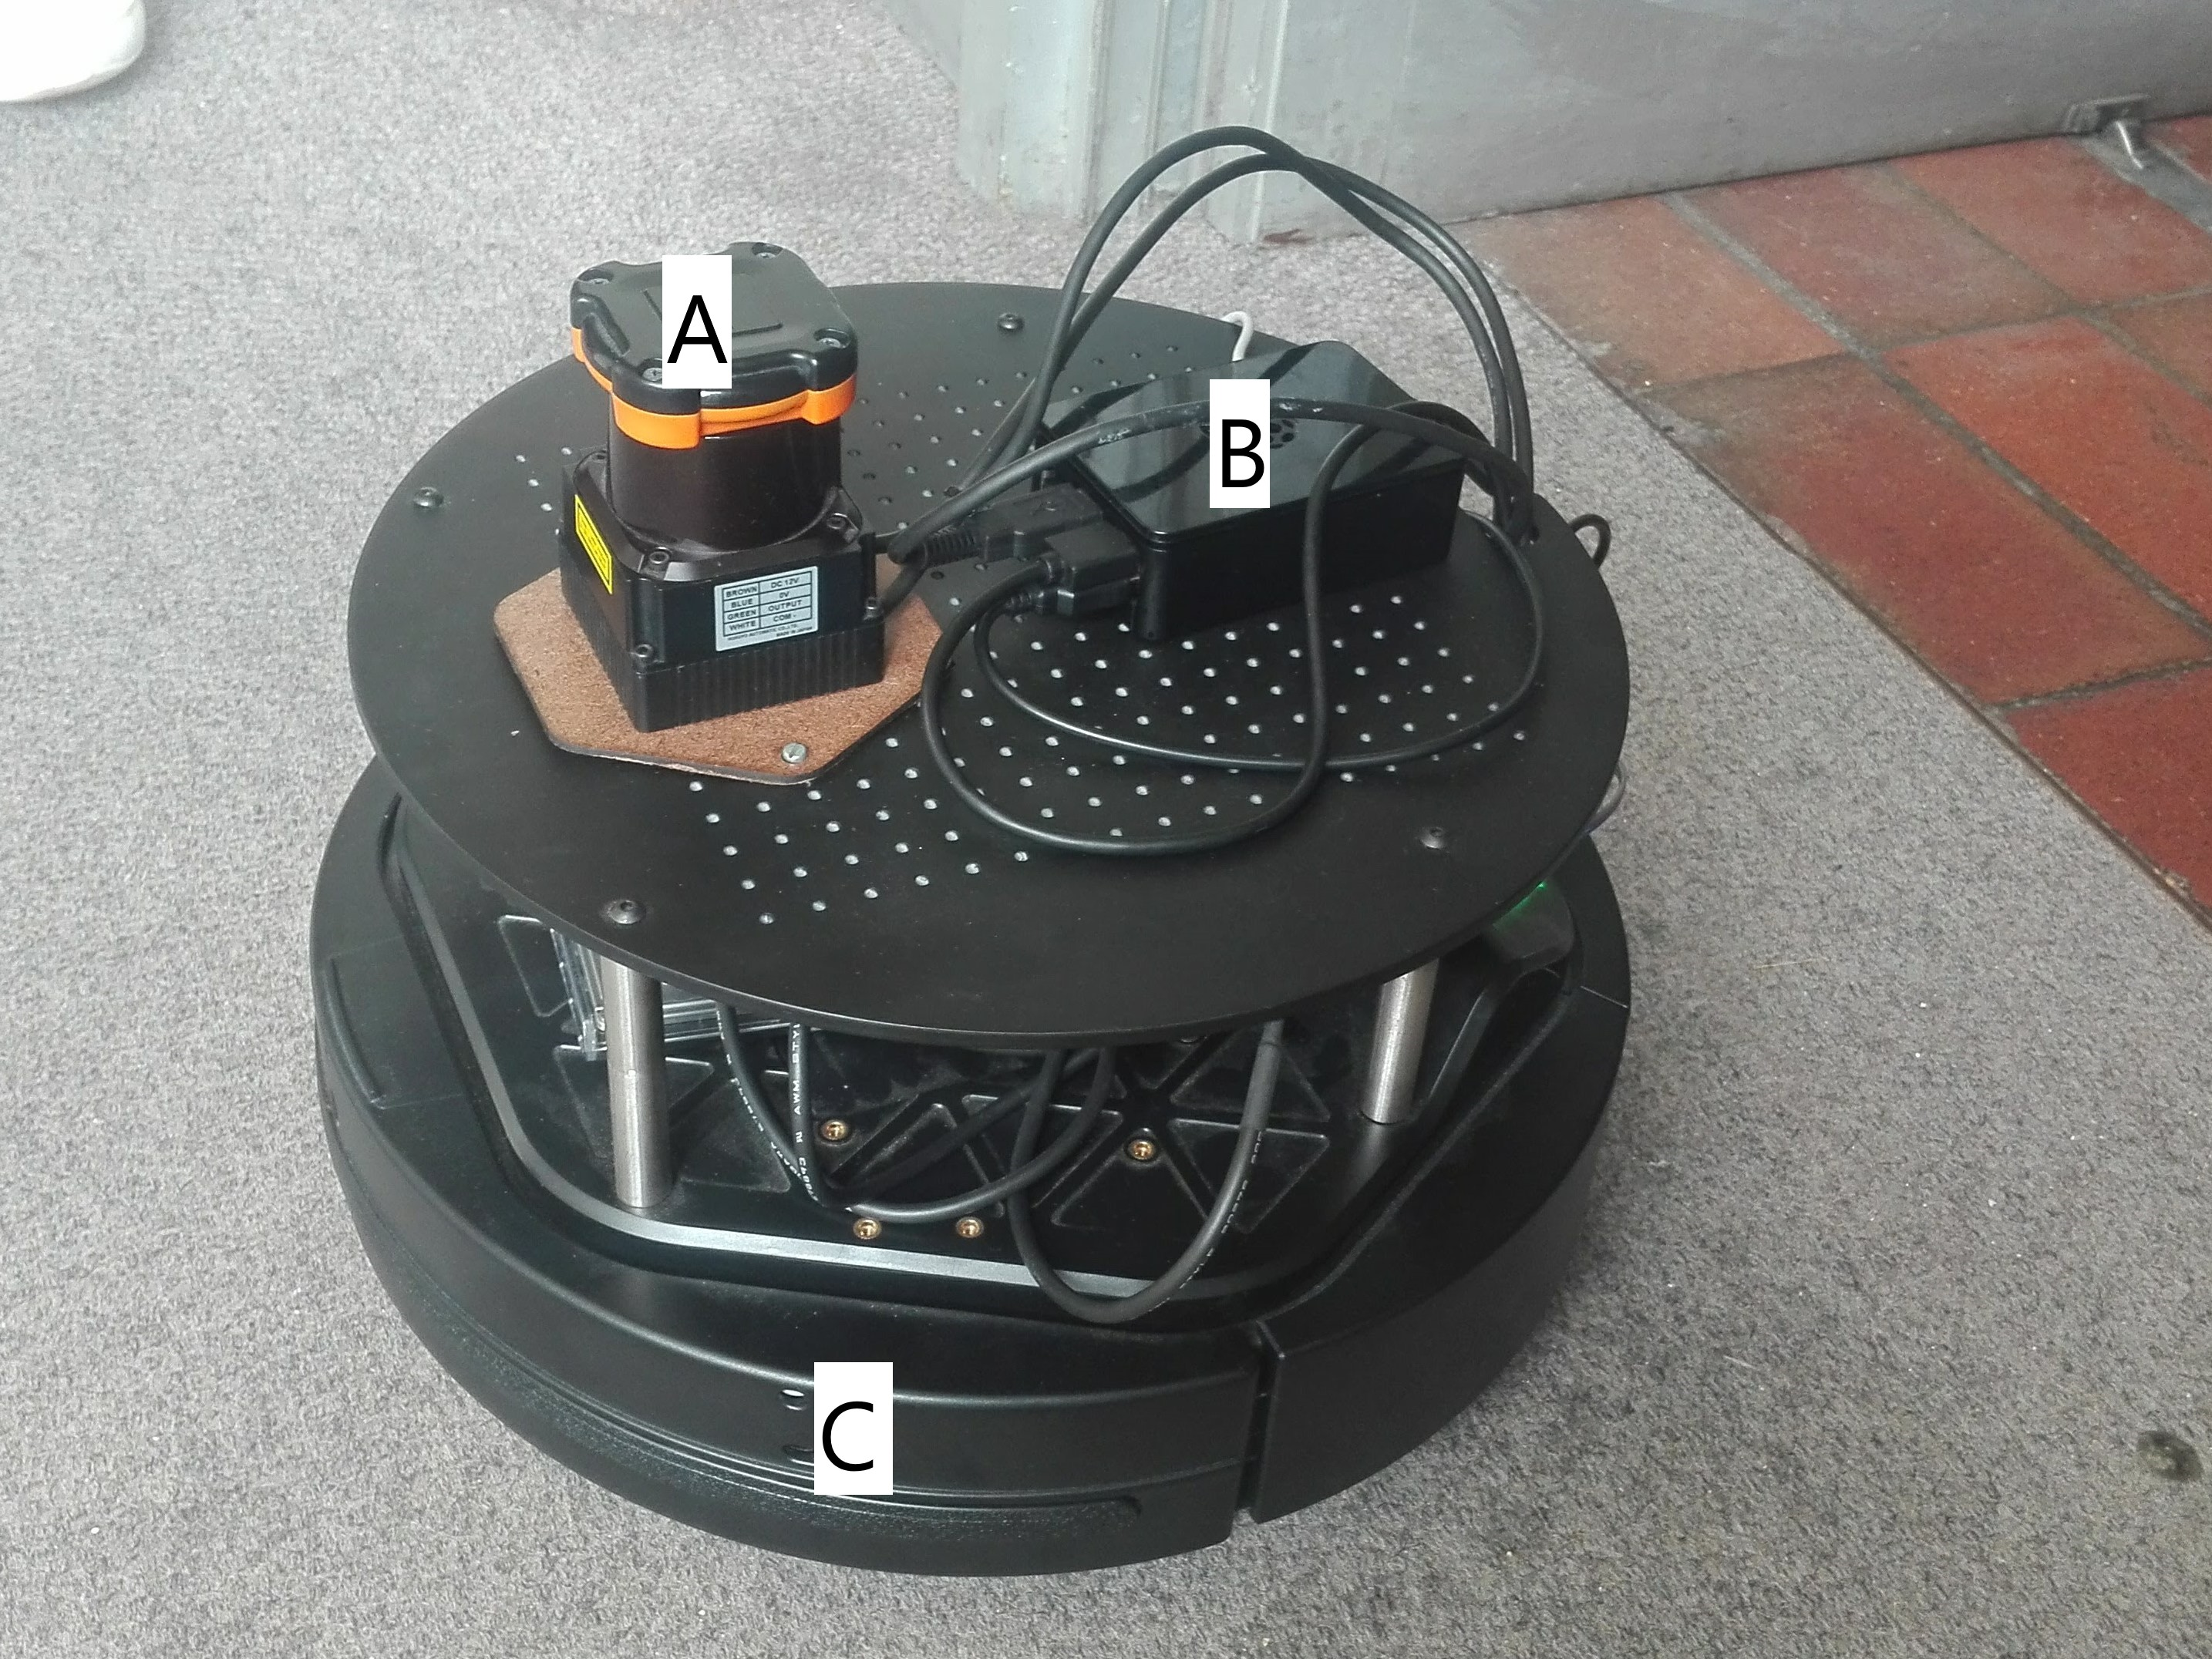
\includegraphics[width=1\textwidth]{figs/real_world_results/turtle_bot.jpg}
    \caption{This figure shows the Kobuki Platform (C) used in the experiments. The platform is equipped with a  Hokuyo UTM-30LX (A) and a Raspberry Pi 3B (B) with ROS installed.}
    \label{fig:turtle_bot_experiments}
\end{figure}


%The chassis is equipped with the following:
%\begin{itemize}
%\item \textbf{Power Connectors}: 19V/2A, 12V/5A, 12v/1.5A and 5V/1A
%\item \textbf{Status Indicator LED}: Green - On, Orange- On but battery low, Green blinking - Battery charging %and if off the platform is off
%\item \textbf{Two Programmable LEDs}
%\item \textbf{USB Port}: For firmware update and platform communication
%\item \textbf{Three Touch Buttons}: These buttons can be used to as inputs
%\item \textbf{Firmware switch}: Enable/disables the firmware update mode
%\item \textbf{Battery}: Lithium-Ion, 14.8V, 2200 mAh (4S1P - small), 4400 mAh (4S2P - large)
%\item \textbf{Motor Overload Detection}: disables power on detecting high current (>3A)
%\item \textbf{Odometry}: 52 ticks/enc rev, 2578.33 ticks/wheel rev, 11.7 ticks/mm
%\item \textbf{Gyro}: factory calibrated, 1 axis (110 deg/s)
%\item \textbf{Bumper Sensors}: left, center, right
%\item \textbf{Cliff Sensors}: left, center, right
%\item \textbf{Wheel Drop Sensor}: left, right
%\item \textbf{Expansion Pins}: 3.3V/1A, 5V/1A, 4 x analogue in, 4 x digital in, 4 x digital out
%\item \textbf{Audio} : several programmable beep sequences
%\item \textbf{Sensor Data Rate}: 50Hz
%\end{itemize}

%====================================================
\subsubsection{Hokuyo UTM-30LX}
\label{sec:hokuyo}
%----------------------------------------------------

Attached to the Kobuki platform is a Hokuyo UTM-30LX (see Figure \ref{fig:hokuyo}), this is a dedicated laser range finder (LIDAR) used in many robotic applications. The sensor requires a 12 volts direct current power supply that can operate between 0.7 amperes and 1 amperes. This sensor uses a semiconductor laser diode with a wavelength (\(\lambda\)) of 905 nanometers. The Field of View (FOV) of the sensor is 270\(\degree\); hence the sensor will typically be mounted on top of the robot to maximise unobstructed FOV. The sensor has an accuracy of 30 millimetres at a range of 0.1 metres to 10 metres, and an accuracy of 50 millimetres at a range of 10 metres to 30 metres. This accuracy can be less reliable if the sensor receives intense light, such as sunlight directly in the outdoor environment. The sensor has an angular resolution of 0.25\(\degree\); this is the minimum angle between different objects in a scan. The sensor is equipped with a USB2.0 connector for communication with other devices.

\begin{figure}[H]
    \centering
    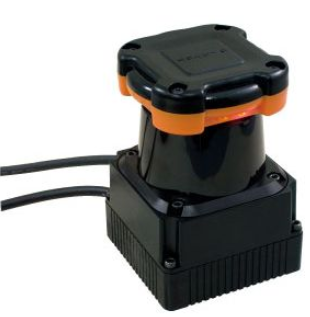
\includegraphics[width=0.3\textwidth]{figs/Hokuyo.png}
    \caption[Hokuyo UTM-30LX LIDAR]{Hokuyo UTM-30LX. Taken from \footnote{https://www.hokuyo-usa.com/products/scanning-laser-rangefinders/utm-30lx}}
    \label{fig:hokuyo}
\end{figure} 

%====================================================
\subsubsection{System integration}
%----------------------------------------------------

The Kobuki Platform is ROS compatible, which is installed on a Raspberry Pi 3B. ROS package turtlebot\_create\footnote{https://github.com/turtlebot/turtlebot\_create} is also installed to connect to the Kuboki platform, and commands are sent through a USB data connection to the platform. To control the motion of the platform and a Logitech F710 wireless gamepad (Figure \ref{fig:logitech_controller} alongside the ROS package \(turtlebot\_teleop\)\footnote{http://wiki.ros.org/turtlebot\_teleop} are used.
 

\begin{figure}[H]
    \centering
    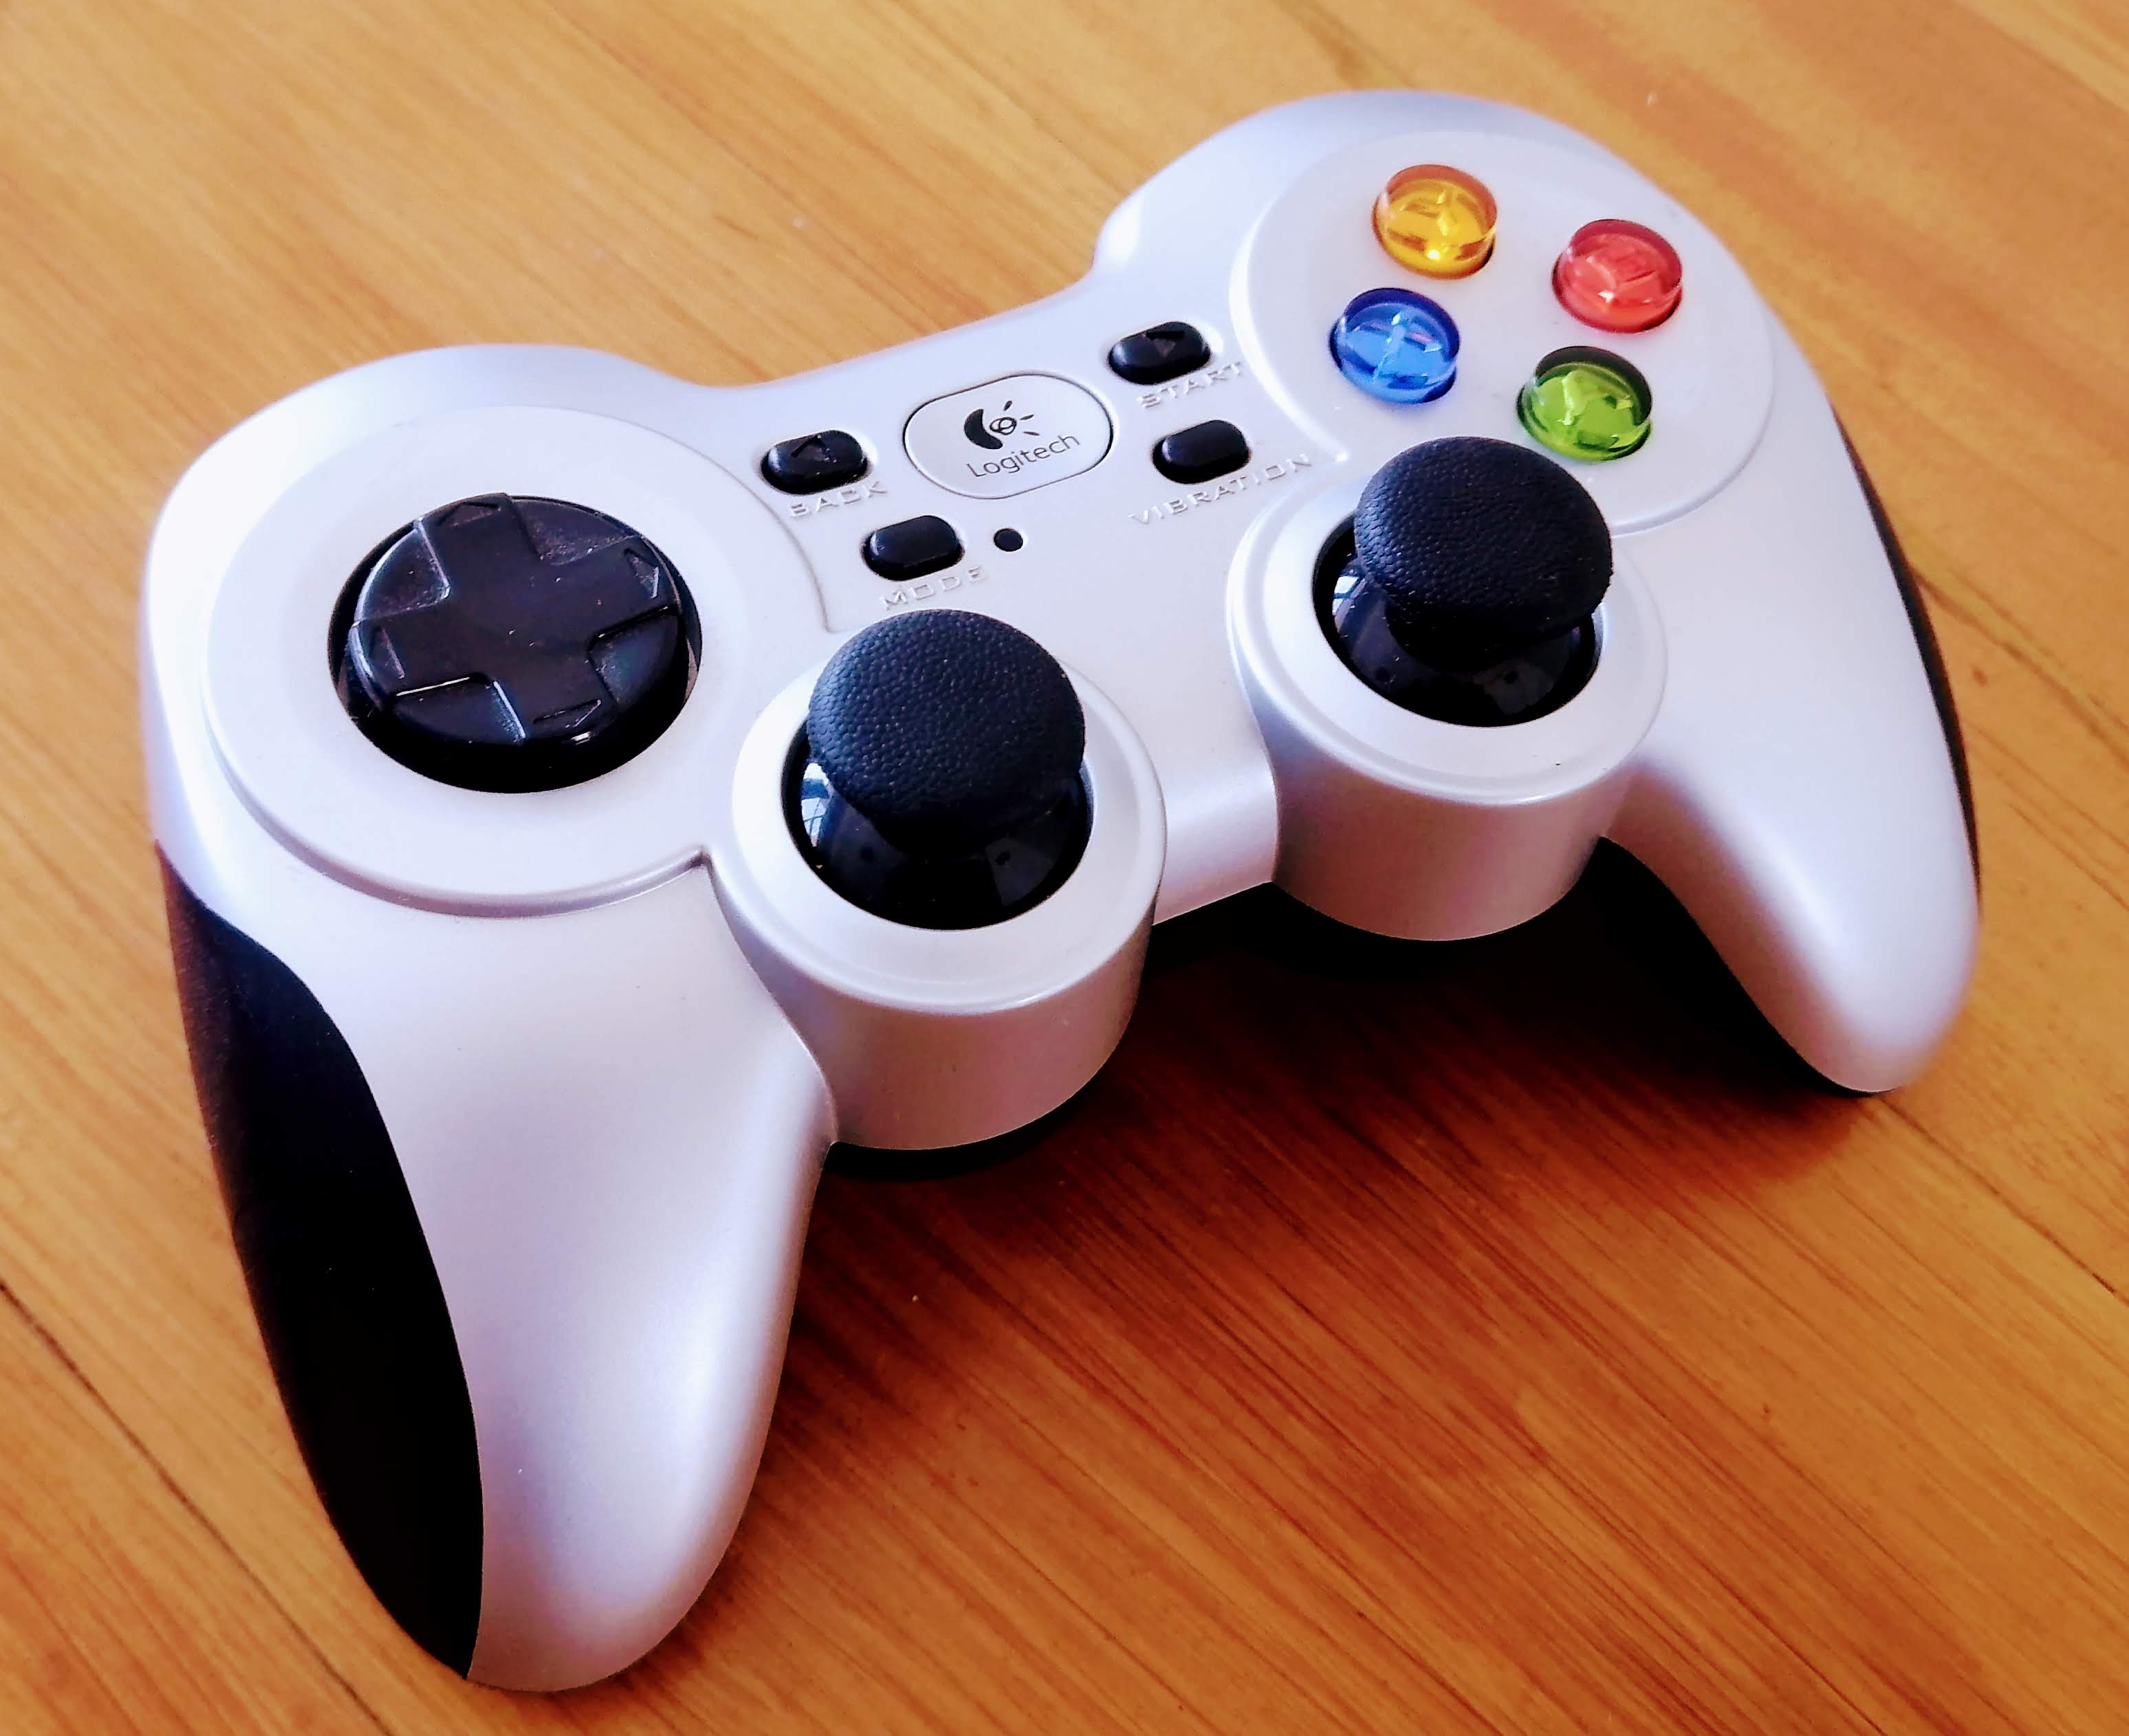
\includegraphics[width=0.3\textwidth]{figs/real_world_results/logitech_controller.jpg}
    \caption{The Logitech Wireless Gamepad F710 uses a powerful and reliable cable-free 2.4 GHz connection while dual-motor vibration and is used to control the Kobuki Platform.}
    \label{fig:logitech_controller}
\end{figure}


%====================================================
\subsection{Results and discussion}
%----------------------------------------------------

In this section, results from real-world data are presented.

%==================================================== 
\subsubsection{Experiment one} %----------------------------------------------------

Figures \ref{fig:real11} and \ref{fig:real12} represents local partial maps from two robots. The local partial maps both have a resolution of 0.05 m/cell. Figure \ref{fig:real13} presents the global map with a resolution of 0.05 m/cell after the alignment and merging of the two partial maps. 

%....................................................
\begin{figure}[H]
\begin{subfigure}{0.5\textwidth}
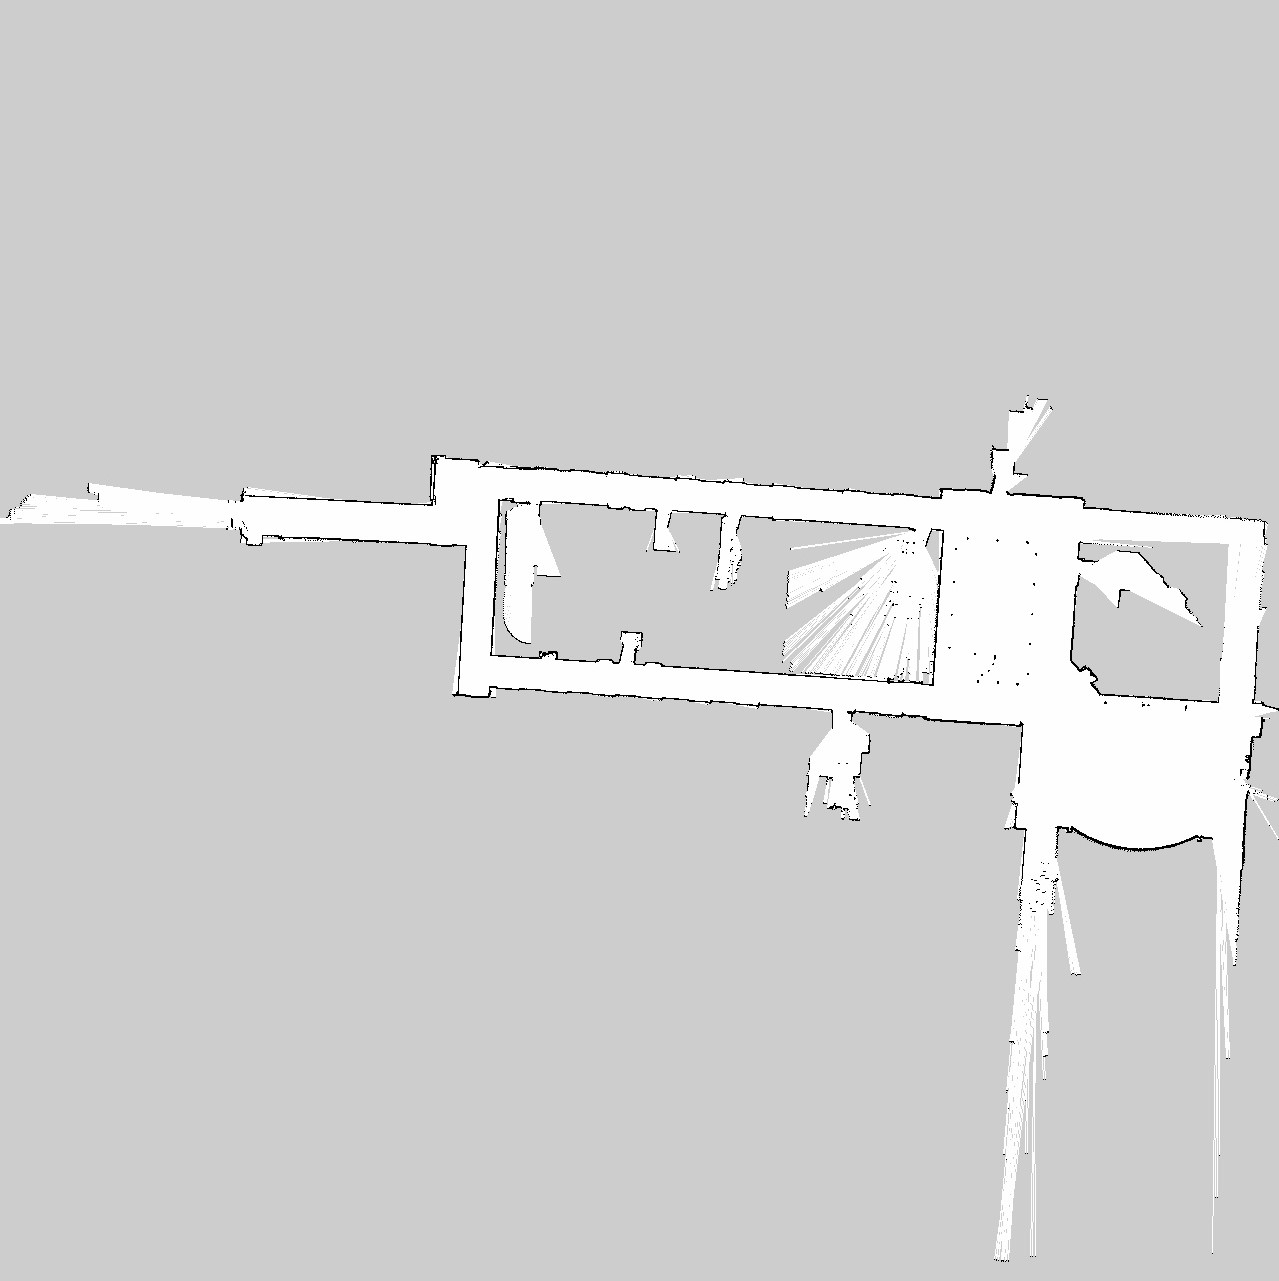
\includegraphics[width=0.9\linewidth, height=5cm]{figs/real_world_results/b/partial_map_1.jpg} 
\caption{Partial map\_1 with resolution of 0.05 m/cell}
\label{fig:real11}
\end{subfigure}
\begin{subfigure}{0.5\textwidth}
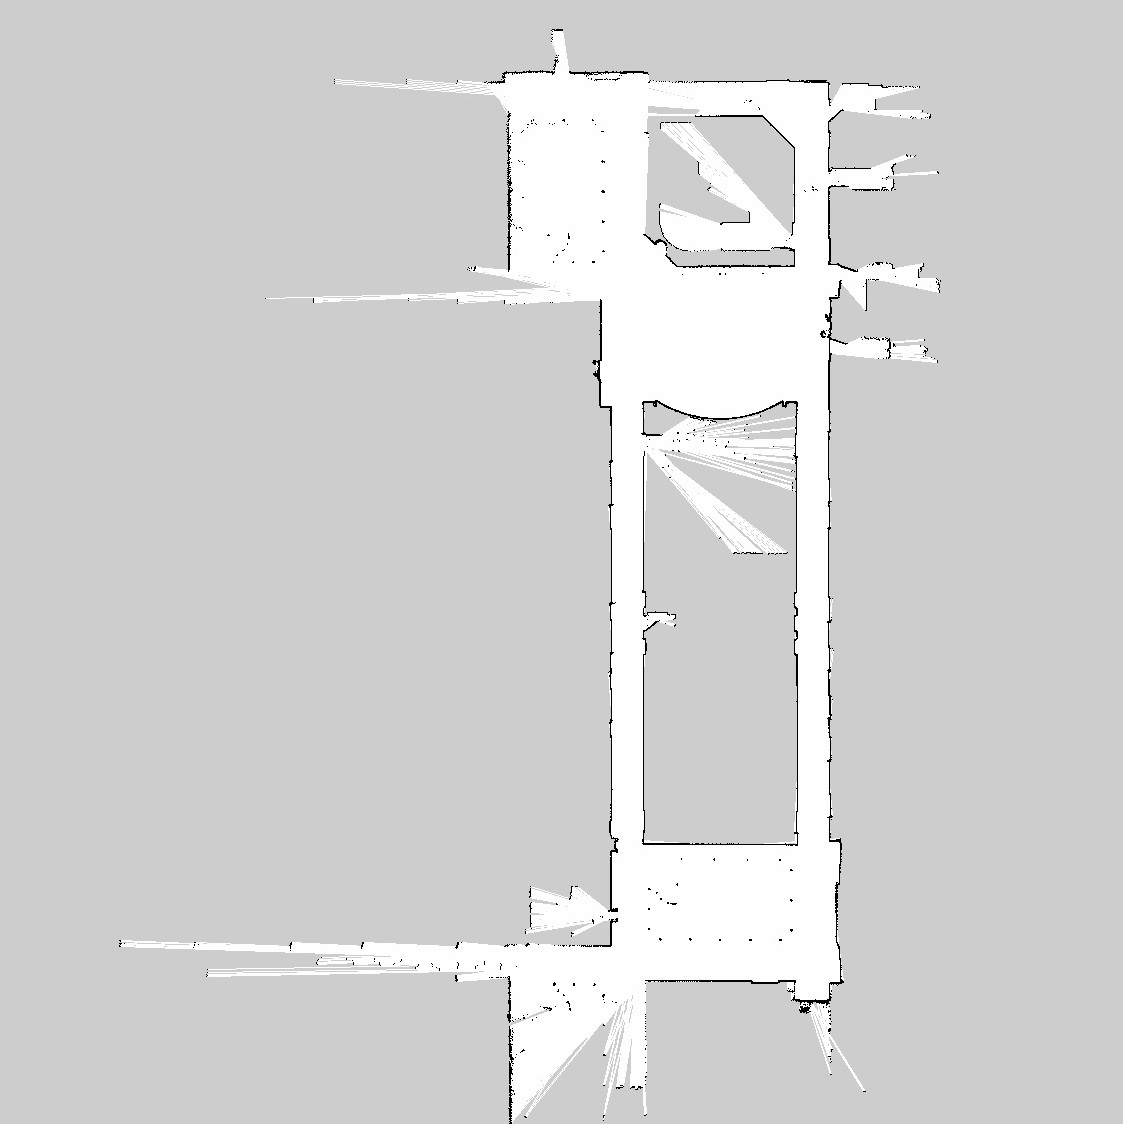
\includegraphics[width=0.9\linewidth, height=5cm]{figs/real_world_results/b/partial_map_2.jpg} 
\caption{Partial map\_2 with resolution of 0.05 m/cell}
\label{fig:real12}
\end{subfigure}
\begin{subfigure}{0.5\textwidth}
\centering
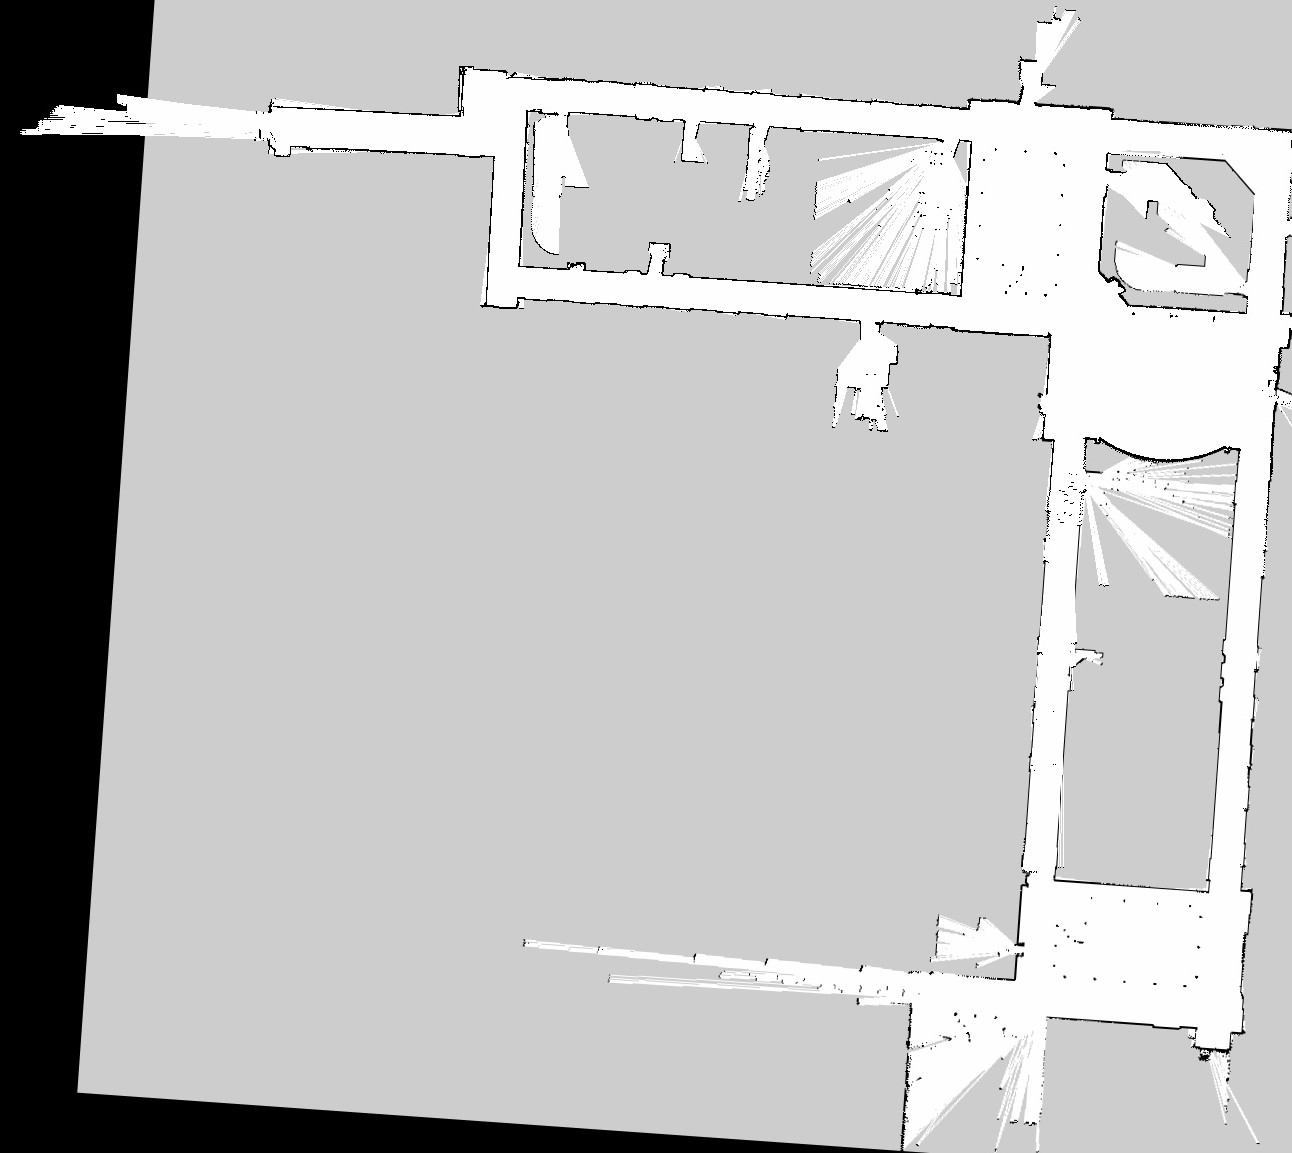
\includegraphics[width=0.9\linewidth, height=5cm]{figs/real_world_results/b/final_map.jpg} 
\caption{Global map with a resolution of 0.05 m/cell}
\label{fig:real13}
\end{subfigure}
\caption{Two partial maps and a global map are presented. The partial maps are generated from real-world data. Since the maps are aligned relative to map\_1, the resultant global map will have the same resolution as partial map\_1.}
\label{fig:real1}
\end{figure}
%....................................................

The new resolution of partial\_map\_2 is within 1\% of partial\_map\_1's resolution (shown in Table \ref{table:real1}), therefore validating the success of the alignment operation. Figure \ref{fig:real1matches1} presents the matched features between the two partial maps, within the 29.78\% overlap region. There are 254 matched features with a match ratio of 0.50. There are significantly more features matched here than in the simulation environment. This result is due to the differing sizes of the maps. The real-world environment is larger than the simulation environment. 

%....................................................
\begin{figure}[H]
    \centering
    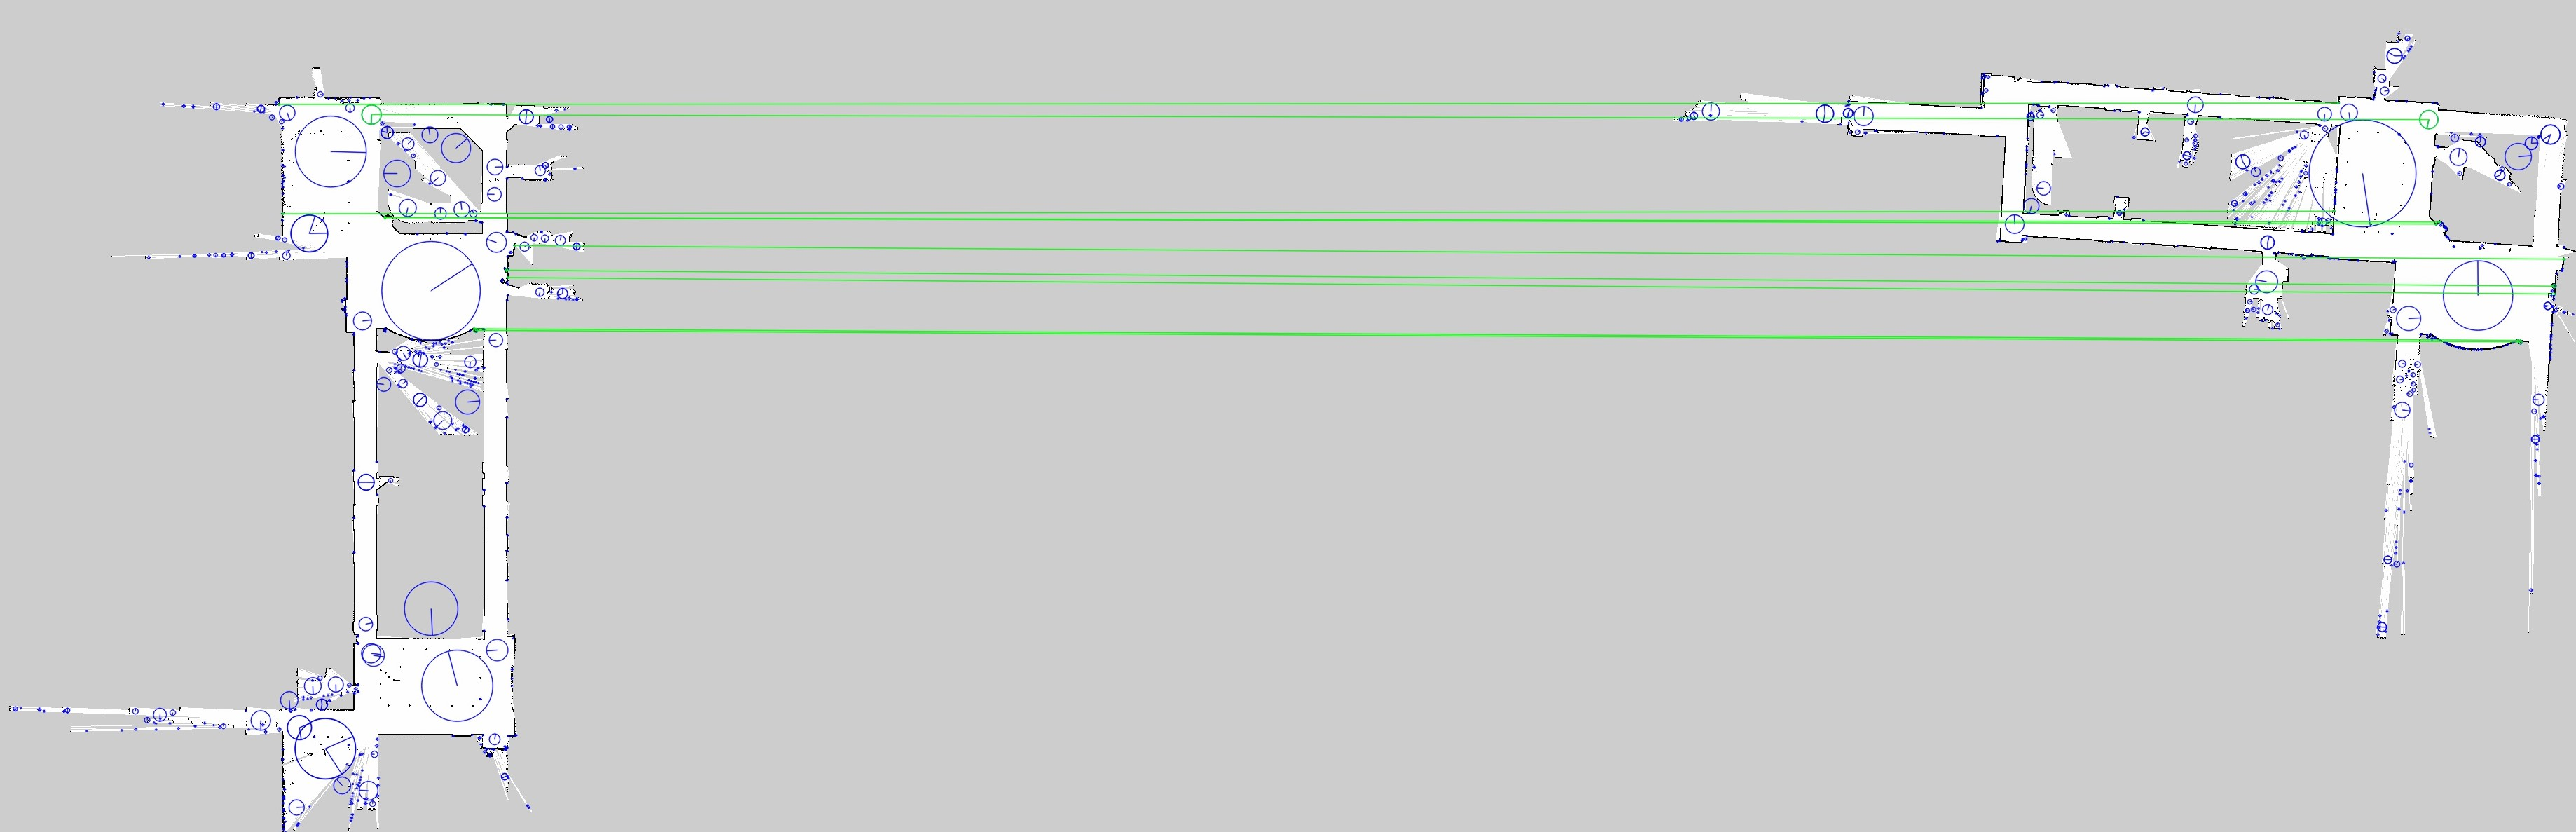
\includegraphics[width=1\textwidth]{figs/real_world_results/b/matchesPartialMap1Map2.jpg}
    \caption{The matched features between partial map\_1 and map\_2 are presented in this figure. The features highlighted in green, are the features that have been matched between the two maps}
    \label{fig:real1matches1}
\end{figure} 
%....................................................

%....................................................
\begin{table}[H]
\centering
\caption{This table presents the results from the alignment and merging operation. Since the partial maps are merged relatively to map\_1 the results are relative to map\_1, which  has a resolution of 0.05 m/cell.}
\begin{tabular}{ | m{1.4cm} | m{2.2cm} | m{2.2cm} | m{2.4cm} | m{1.7cm} | m{1.4cm} | m{2.4cm} | }
\hline
\textbf{Map} & \textbf{Resolution (m/cell)} & \textbf{New resolution (m/cell)} & \textbf{Angle of rotation (\degree)} & \textbf{Good matches} & \textbf{Match ratio} & \textbf{Percentage overlap}\\ 
\hline
\hline
Partial map\_2  & 0.05  & 0.049870607 & -4.048134489 & 254 & 0.50 & 29.78\\ 
\hline
\end{tabular}
\label{table:real1}
\end{table}
%....................................................


%==================================================== 
\subsubsection{Experiment two} %----------------------------------------------------

Figures \ref{fig:real21}, \ref{fig:real22} and \ref{fig:real23} represent three partial local maps from robots, before the alignment and merging process. The partial maps have the same resolution of 0.1 m/cell. Figure \ref{fig:real24} presents the global map with a resolution of 0.1 m/cell after the alignment and merging of the three partial maps. Furthermore, note that: Figure \ref{fig:real24} in the red region, partial map\_2 has a SLAM error which is evident in the global\_map; And Figure \ref{fig:real24} in green region new information from partial map\_3 is now present in the global\_map.

%....................................................
\begin{figure}[H]
\begin{subfigure}{0.5\textwidth}
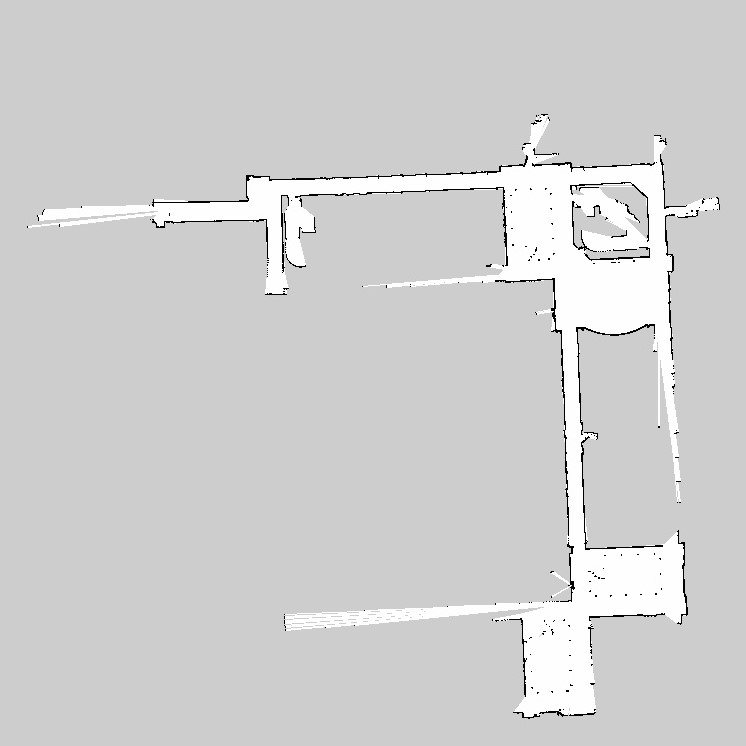
\includegraphics[width=0.9\linewidth, height=5cm]{figs/real_world_results/c/partial_map_1.jpg} 
\caption{Partial map\_1 with a resolution of 0.1 m/cell}
\label{fig:real21}
\end{subfigure}
\begin{subfigure}{0.5\textwidth}
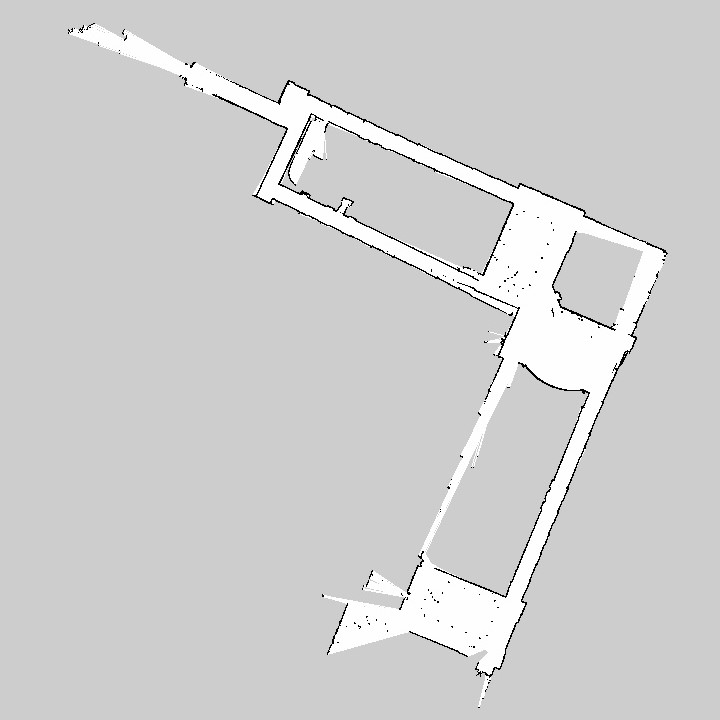
\includegraphics[width=0.9\linewidth, height=5cm]{figs/real_world_results/c/partial_map_2.jpg} 
\caption{Partial map\_2 with a resolution of 0.1 m/cell}
\label{fig:real22}
\end{subfigure}
\begin{subfigure}{0.5\textwidth}
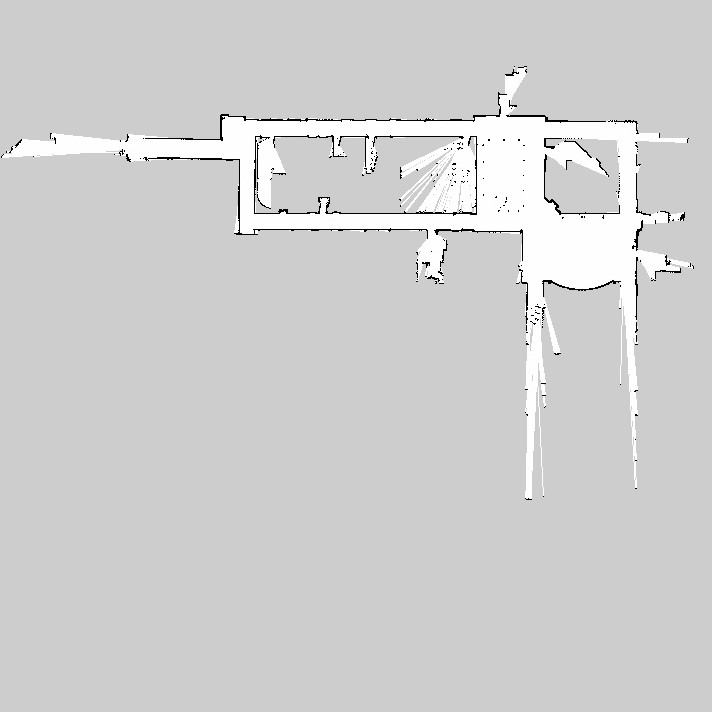
\includegraphics[width=0.9\linewidth, height=5cm]{figs/real_world_results/c/partial_map_3.jpg} 
\caption{Partial map\_2 with a resolution of 0.1 m/cell}
\label{fig:real23}
\end{subfigure}
\begin{subfigure}{0.5\textwidth}
\centering
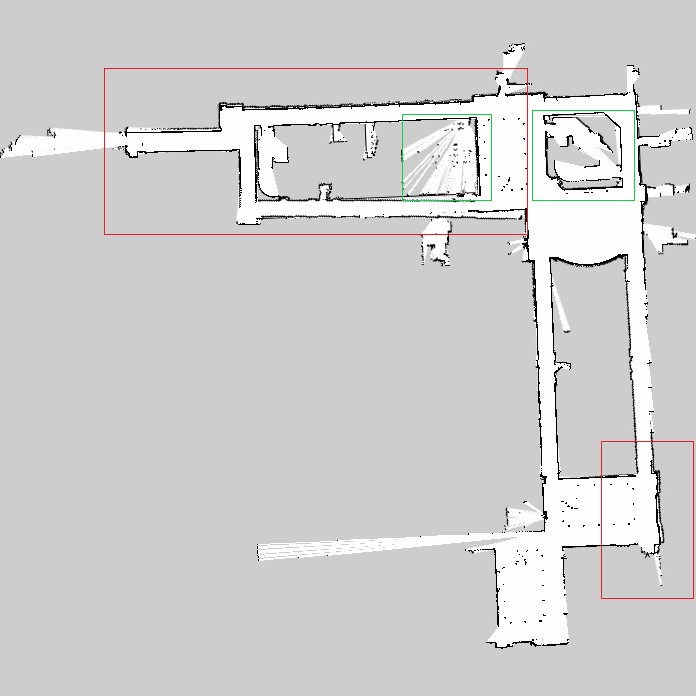
\includegraphics[width=0.9\linewidth, height=5cm]{figs/real_world_results/c/final_map_marked.jpg}
\caption{Global map with a resolution of 0.1 m/cell}
\label{fig:real24}
\end{subfigure}
\caption{Three partial maps and a global map are presented. The partial maps are generated from real-world data. Since the maps are aligned relative to map\_1, the resultant global map will have the same resolution as partial map\_1.}
\label{fig:real2}
\end{figure}
%....................................................

The new resolution of partial\_map\_2 and partial\_map\_3 are within 1\% of partial\_map\_1's resolution (shown in Table \ref{table:real2}), therefore validating the success of the alignment operation. Figure \ref{fig:real2matches1} shows the feature matches between partial map\_1 and map\_2, with a match ratio of 0.61 in an overlap region of 47.47\% (see Table \ref{table:real2}). And Figure \ref{fig:real2matches2} shows the feature matches between partial map\_1 and map\_3, with a match ratio of 0.52 in an overlap region of 37.83\% (see Table \ref{table:real2}). Again here we observe that the match ratio and percentage overlap are directly proportional.

%....................................................
\begin{figure}[H]
    \centering
    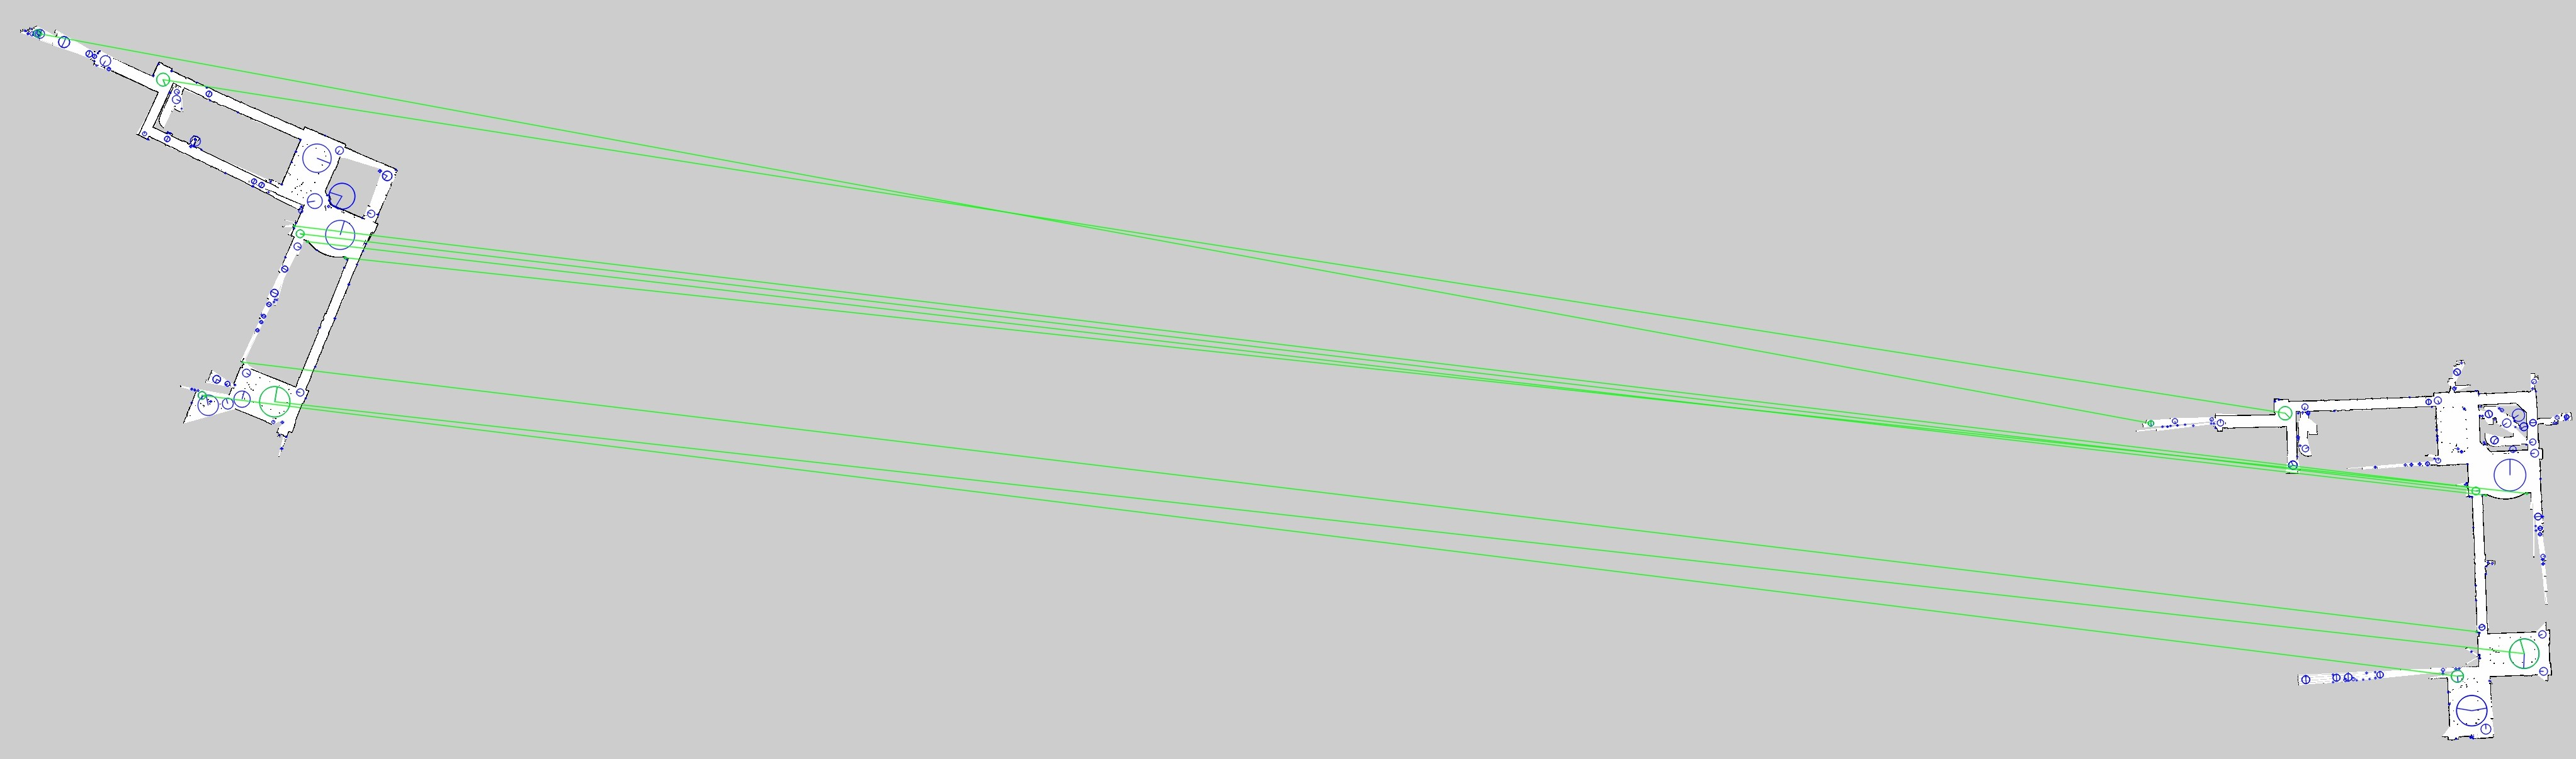
\includegraphics[width=1\textwidth]{figs/real_world_results/c/matchesPartialMap1Map2.jpg}
    \caption{The matched features between partial map\_1 and map\_2 are presented in this figure. The features highlighted in green, are the features that have been matched between the two maps}
    \label{fig:real2matches1}
\end{figure} 
%....................................................


%....................................................
\begin{figure}[H]
    \centering
    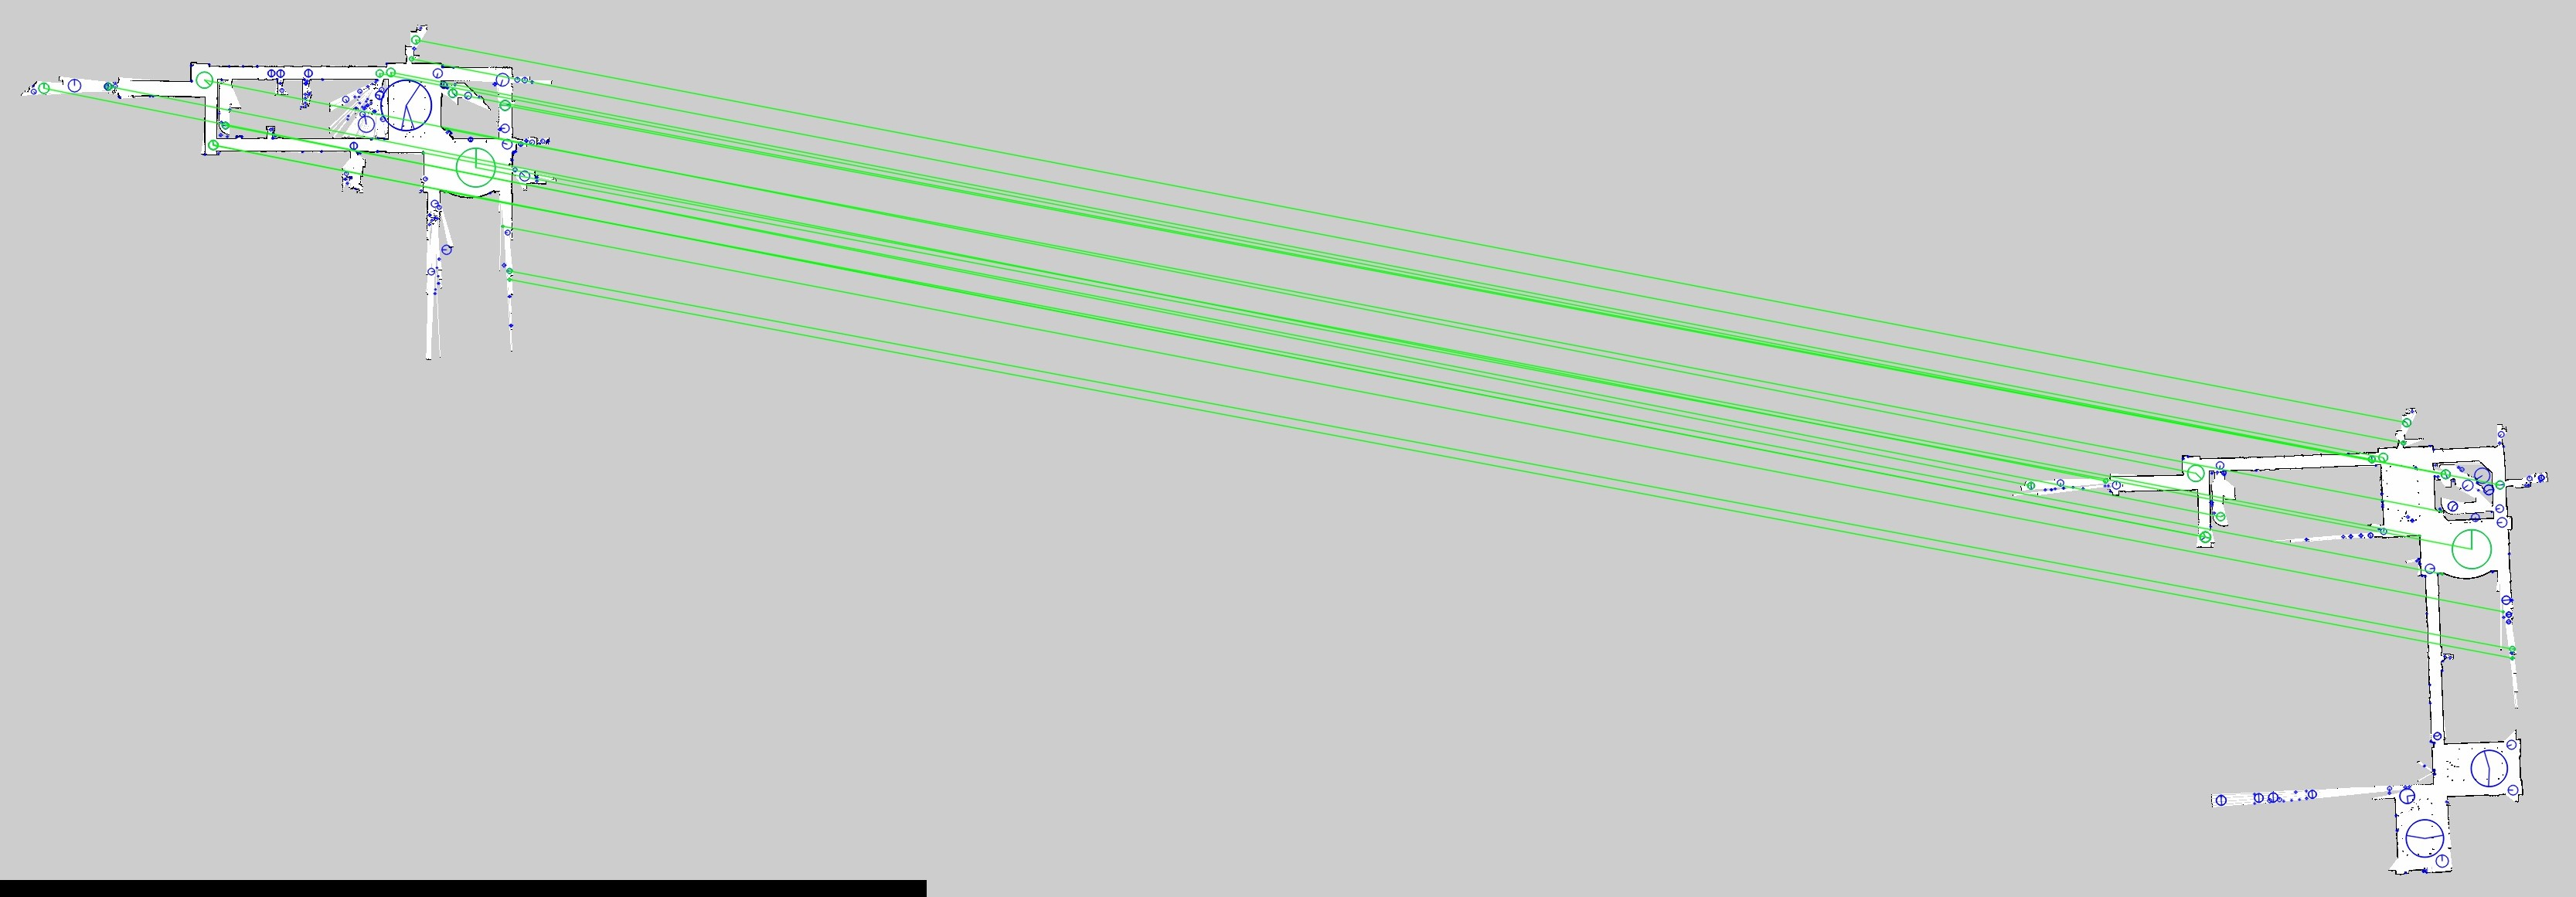
\includegraphics[width=1\textwidth]{figs/real_world_results/c/matchesPartialMap1Map3.jpg}
       \caption{The matched features between partial map\_1 and map\_3 are presented in this figure. The features highlighted in green, are the features that have been matched between the two maps}
    \label{fig:real2matches2}
\end{figure} 
%....................................................



%....................................................
\begin{table}
\centering
\caption{This table presents the results from the alignment and merging operation. Since the partial maps are merged relatively to map\_1 the results are relative to map\_1, which  has a resolution of 0.1 m/cell.}
\begin{tabular}{ | m{1.4cm} | m{2.2cm} | m{2.2cm} | m{2.4cm} | m{1.7cm} | m{1.4cm} | m{2.4cm} | }
\hline
\textbf{Map} & \textbf{Resolution (m/cell)} & \textbf{New resolution (m/cell)} & \textbf{Angle of rotation (\degree)} & \textbf{Good matches} & \textbf{Match ratio} & \textbf{Percentage overlap}\\ 
\hline
\hline
Partial map\_2  & 0.1  & 0.100179351 & 25.60591752 & 107 & 0.61 & 47.47\\ 
\hline
Partial map\_3  & 0.1  & 0.099236774 & 2.310055427 & 106 & 0.52 & 37.83\\ 
\hline
\end{tabular}
\label{table:real2}
\end{table}
%....................................................


%==================================================== 
\subsubsection{Experiment three} %----------------------------------------------------

Figures \ref{fig:real31}, \ref{fig:real32}, \ref{fig:real33} and \ref{fig:real34} represent four partial local maps from robots, before the alignment and merging process. The partial maps 1, 2 and 3 have the same resolution of 0.05 m/cell, and partial map\_4 has a resolution of 0.1 m/cell. Figure \ref{fig:real35} presents the global map with a resolution of 0.05 m/cell after the alignment and merging of the four partial maps. The global map represents the environment's full map shown in \ref{fig:uct_floor}. In Figure \ref{fig:real35}, the final map has two main areas of interest; green and red regions. The red region shows the propagated SLAM error from partial map\_2 (see Figure \ref{fig:real32}). The green region shows a misalignment of the partial maps, potentially caused by the SLAM error in partial map\_2.


%....................................................
\begin{figure}[H]
\begin{subfigure}{0.5\textwidth}
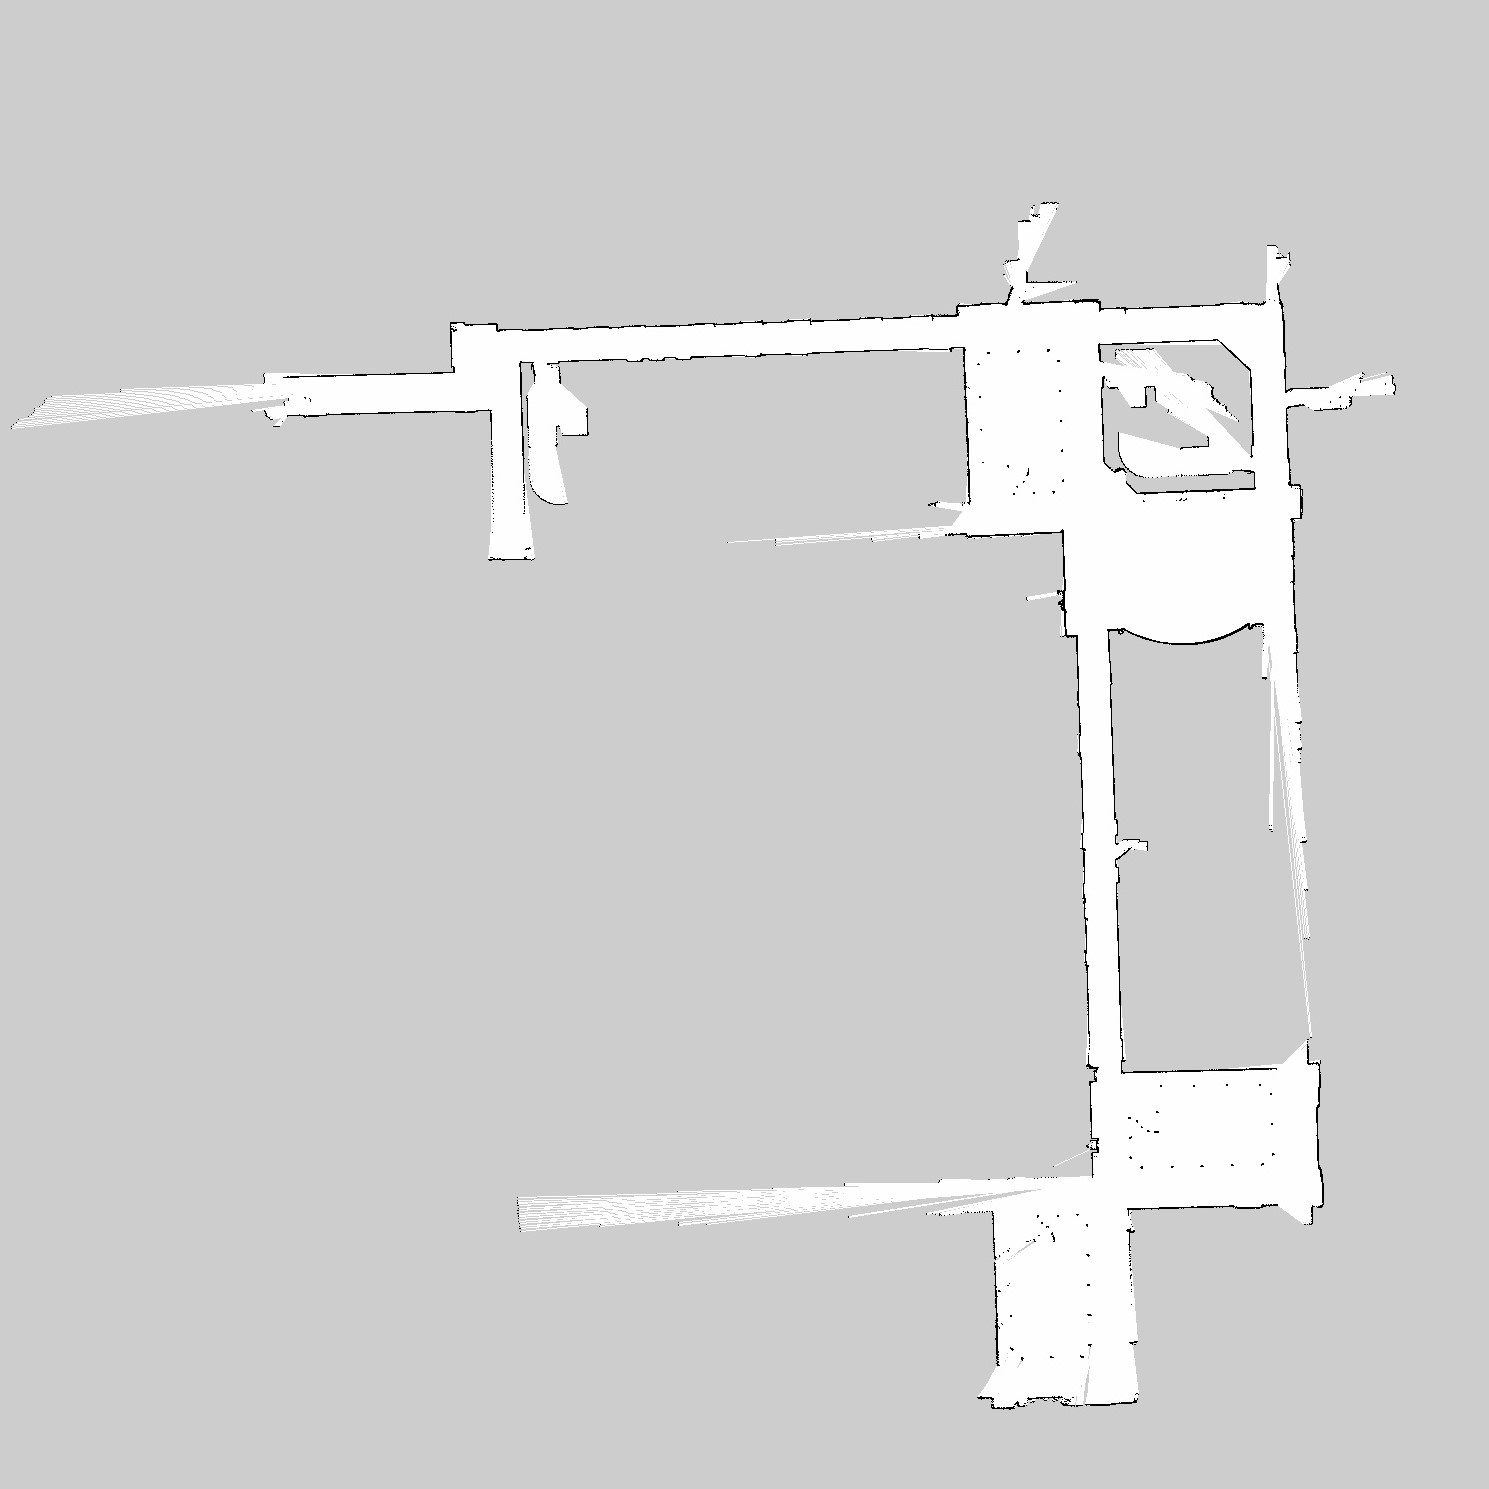
\includegraphics[width=0.9\linewidth, height=5cm]{figs/real_world_results/a/partial_map_1.jpg} 
\caption{Partial map\_1 with resolution of 0.05 m/cell}
\label{fig:real31}
\end{subfigure}
\begin{subfigure}{0.5\textwidth}
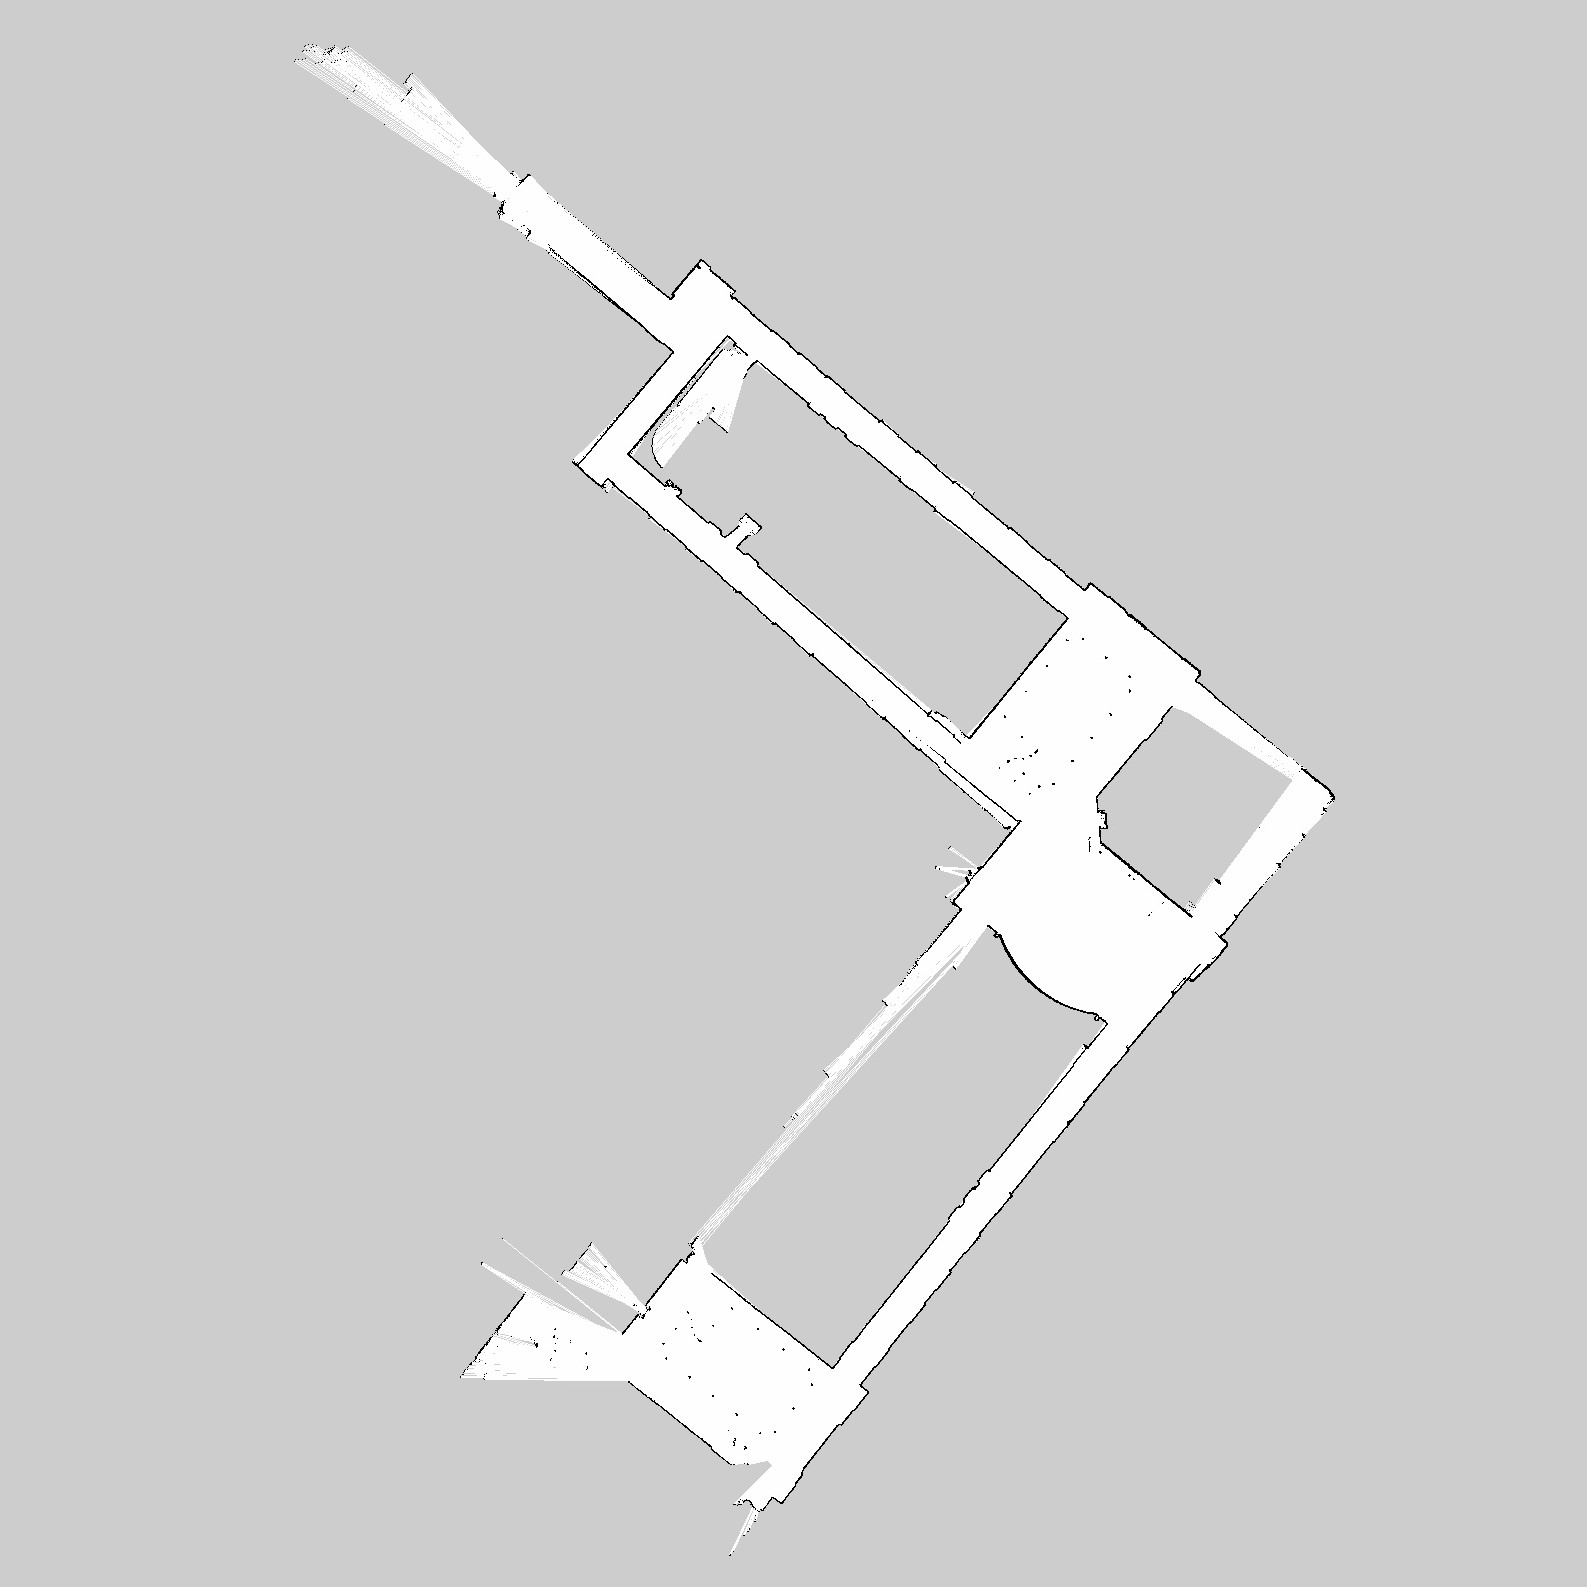
\includegraphics[width=0.9\linewidth, height=5cm]{figs/real_world_results/a/partial_map_2.jpg} 
\caption{Partial map\_2 with resolution of 0.05 m/cell}
\label{fig:real32}
\end{subfigure}
\begin{subfigure}{0.5\textwidth}
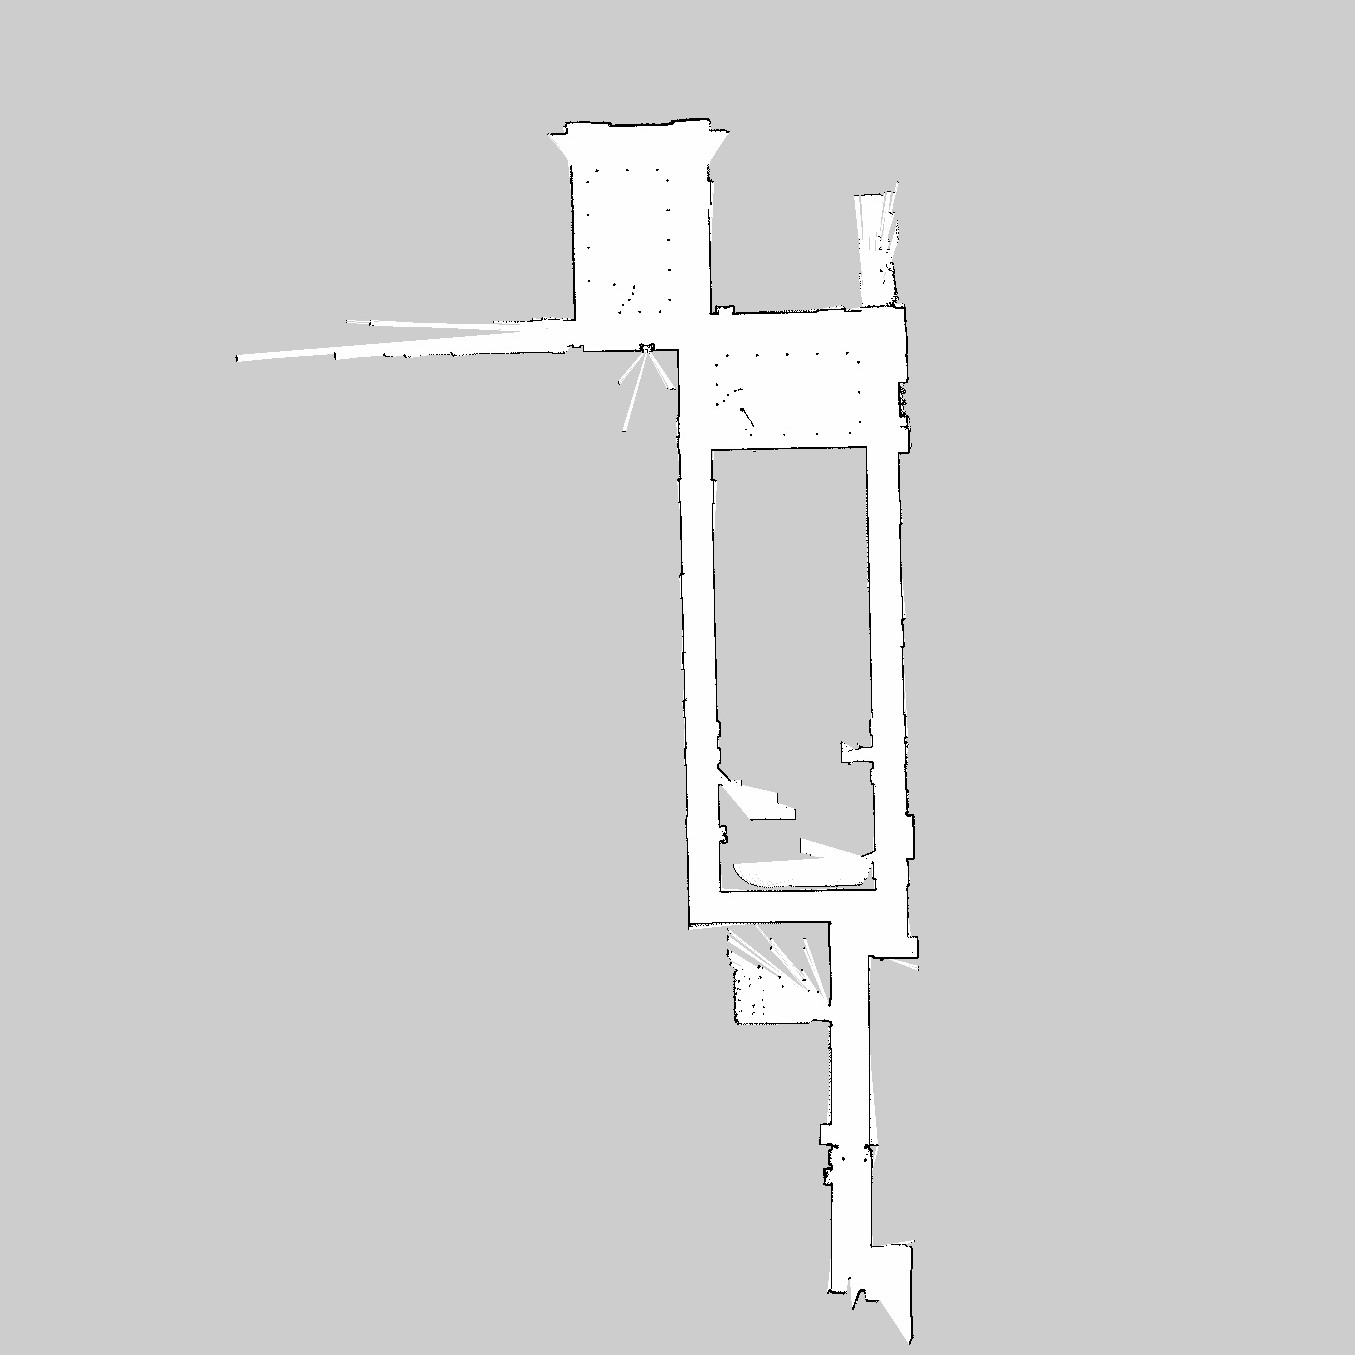
\includegraphics[width=0.9\linewidth, height=5cm]{figs/real_world_results/a/partial_map_3.jpg} 
\caption{Partial map\_3 with resolution of 0.05 m/cell}
\label{fig:real33}
\end{subfigure}
\begin{subfigure}{0.5\textwidth}
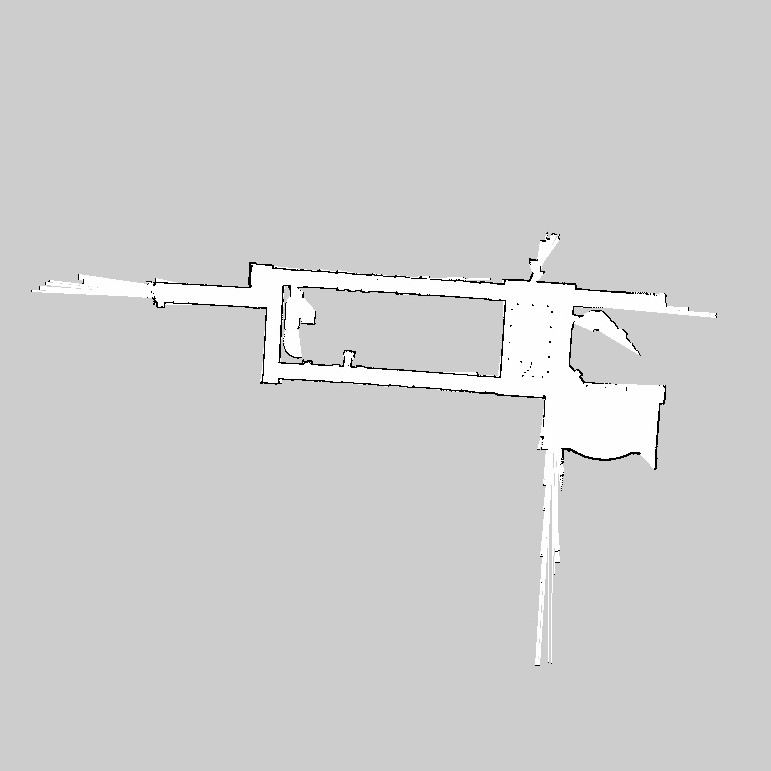
\includegraphics[width=0.9\linewidth, height=5cm]{figs/real_world_results/a/partial_map_4.jpg} 
\caption{Partial map\_3 with resolution of 0.1 m/cell}
\label{fig:real34}
\end{subfigure}
\begin{subfigure}{0.5\textwidth}
\centering
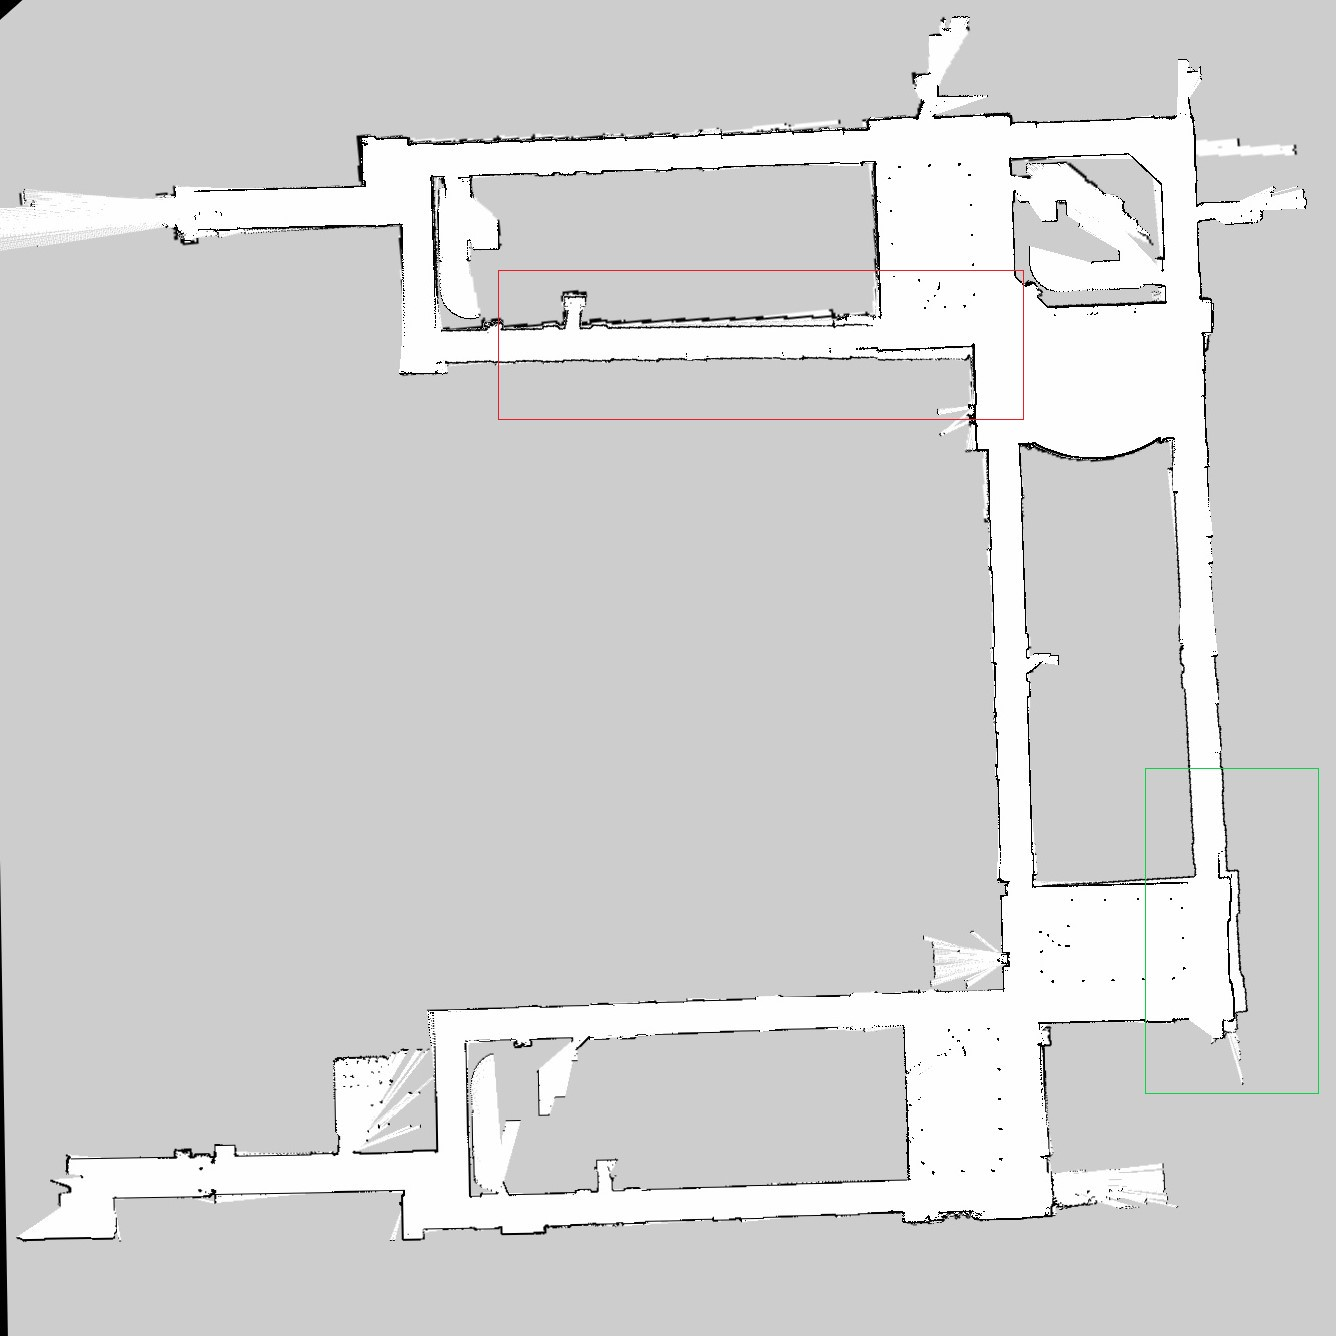
\includegraphics[width=0.9\linewidth, height=5cm]{figs/real_world_results/a/final_map_marked.jpg} 
\caption{Global map with resolution of 0.05 m/cell}
\label{fig:real35}
\end{subfigure}
\caption{Four partial maps and a global map are presented. The partial maps are generated from real-world data. Since the maps are aligned relative to map\_1, the resultant global map will have the same resolution as partial map\_1.}
\label{fig:real3}
\end{figure}
%....................................................

The new resolution of partial\_map\_2, partial\_map\_3 and partial\_map\_4 are with in 1\% of partial\_map\_1's resolution (shown in Table \ref{table:real3}), therefore validating the success of the alignment operation. Figure \ref{fig:real3matches1} shows the feature matches between partial map\_1 and map\_2, with a match ratio of 0.49 in an overlap region of 51.60\% (see Table \ref{table:real3}). Figure \ref{fig:real3matches2} shows the feature matches between partial map\_1 and map\_3, with a match ratio of 0.55 in an overlap region of 23.71\% (see Table \ref{table:real3}). Figure \ref{fig:real3matches2} shows the feature matches between partial map\_1 and map\_4, with a match ratio of 0.91 in an overlap region of 29.37\% (see Table \ref{table:real3}). Here we see that the direct proportionality of match ratio and percentage overlap do not hold.

%....................................................
\begin{figure}[H]
    \centering
    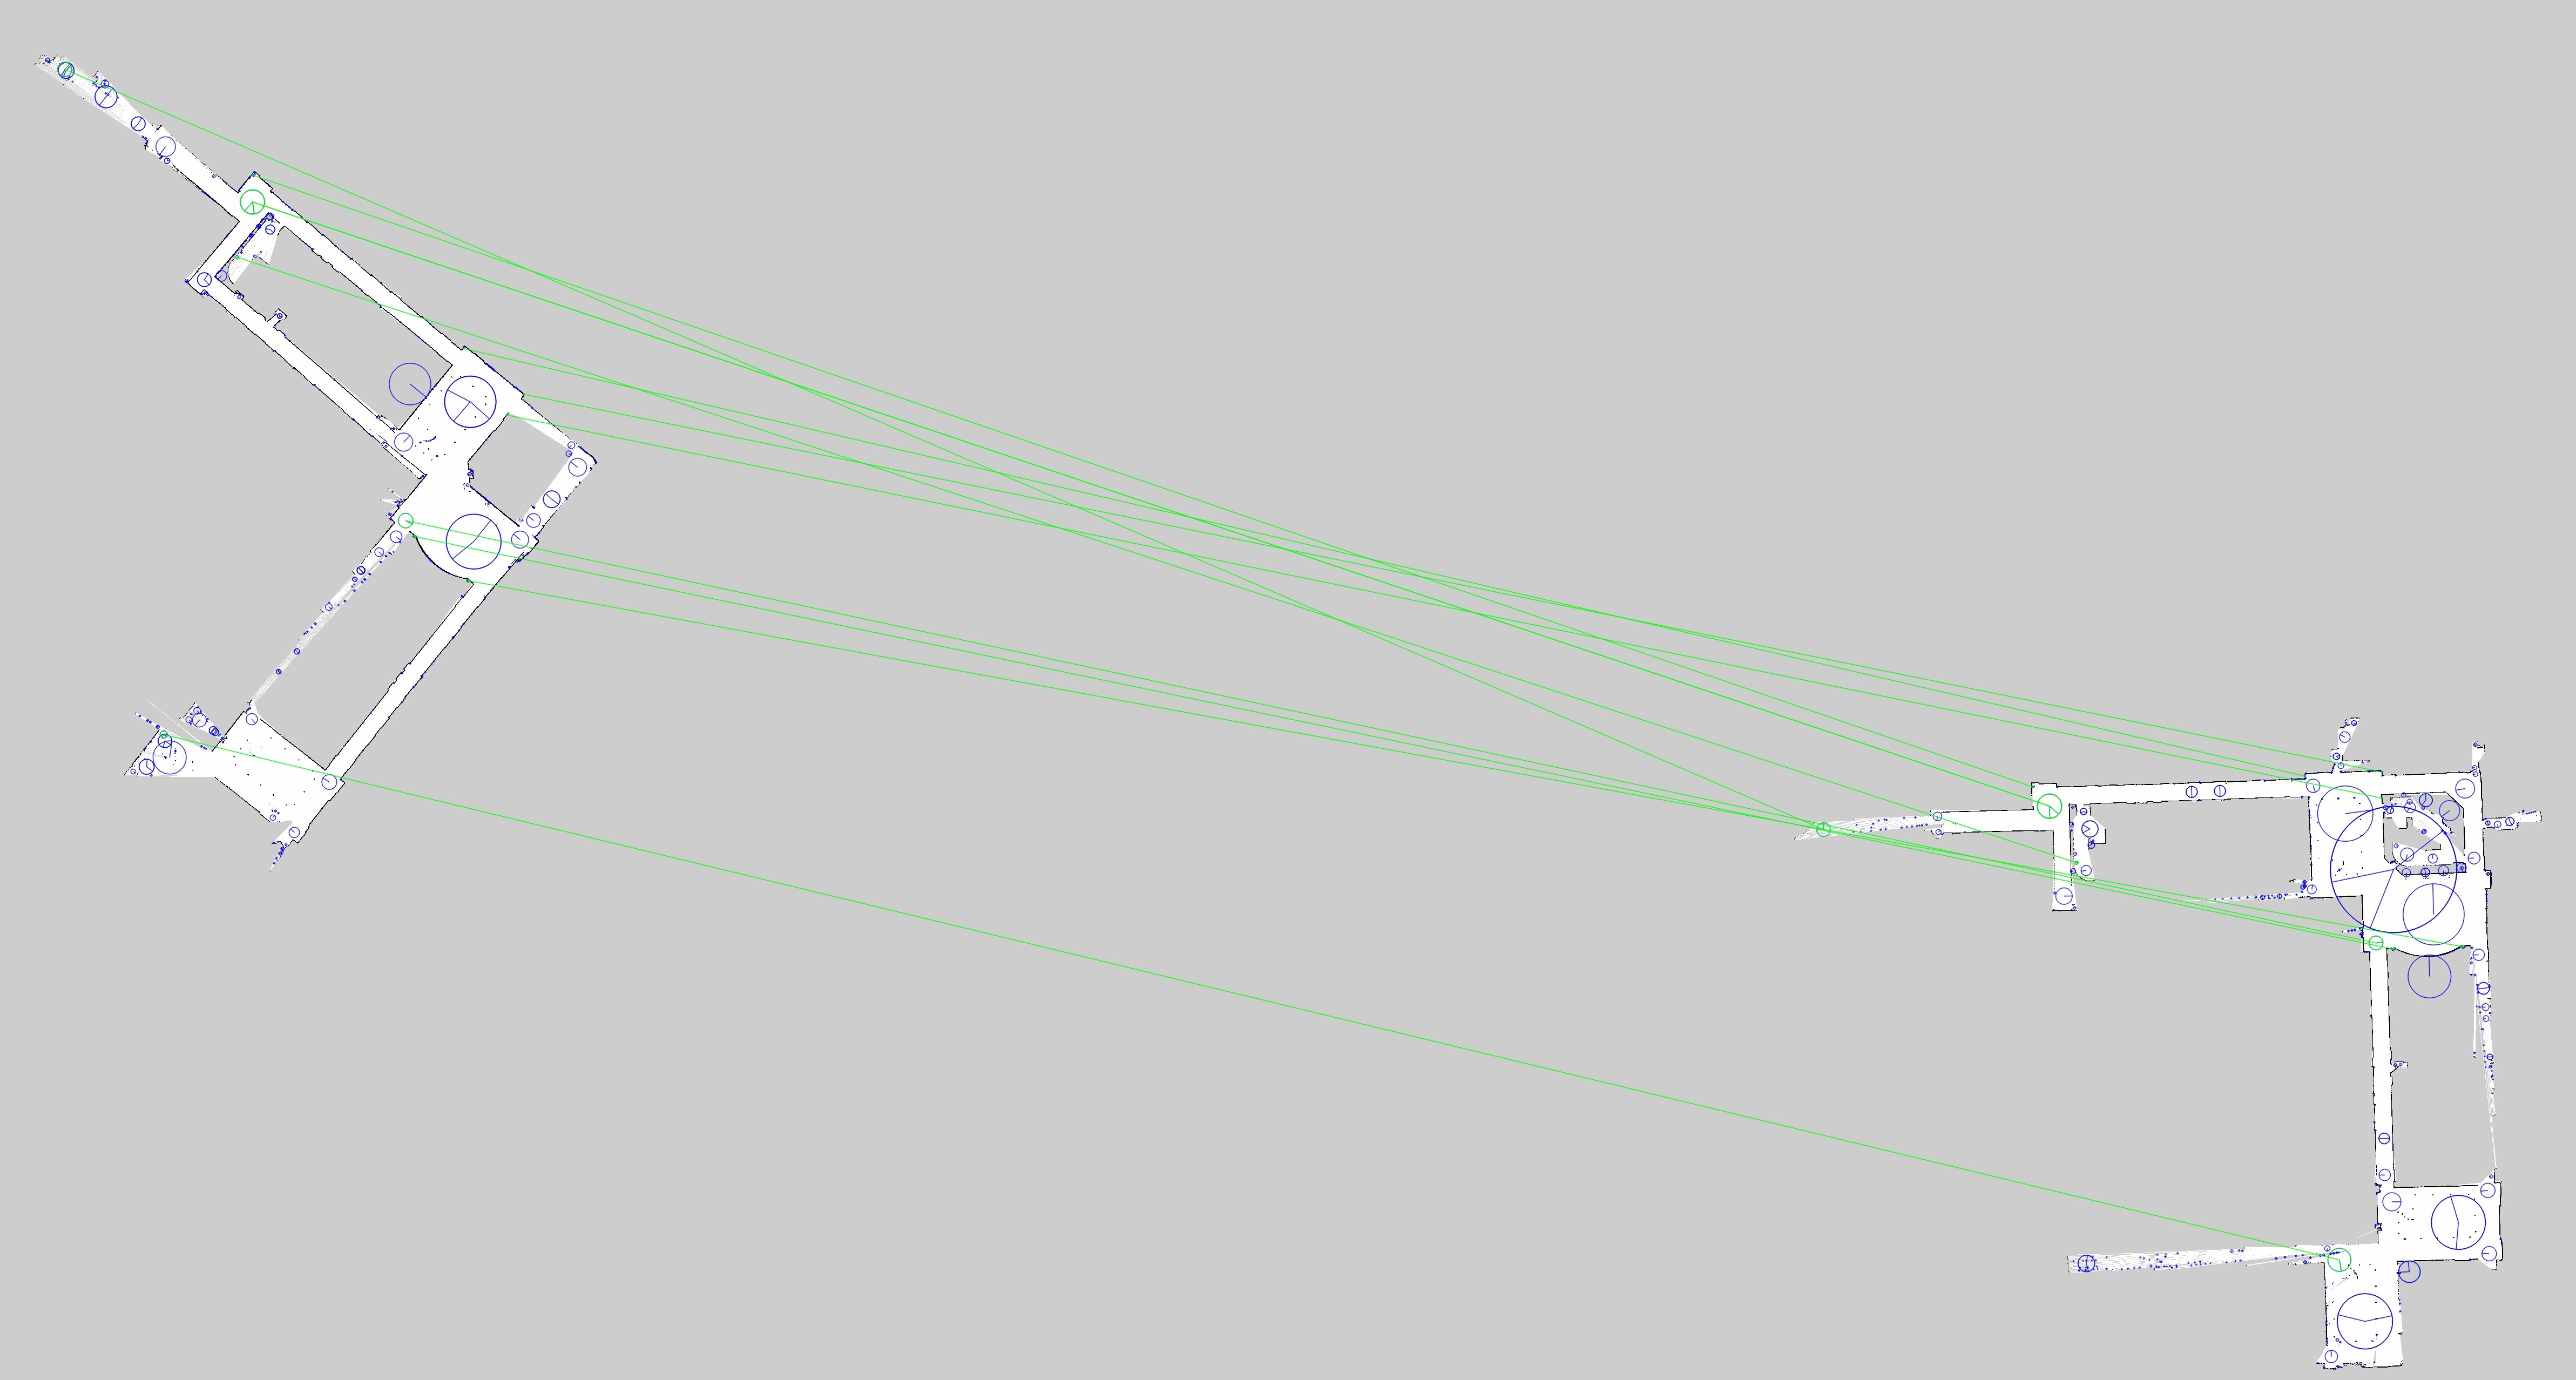
\includegraphics[width=1\textwidth]{figs/real_world_results/a/matchesPartialMap1Map2.jpg}
    \caption{The matched features between partial map\_1 and map\_2 are presented in this figure. The features highlighted in green, are the features that have been matched between the two maps}
    \label{fig:real3matches1}
\end{figure} 
%....................................................


%....................................................
\begin{figure}[H]
    \centering
    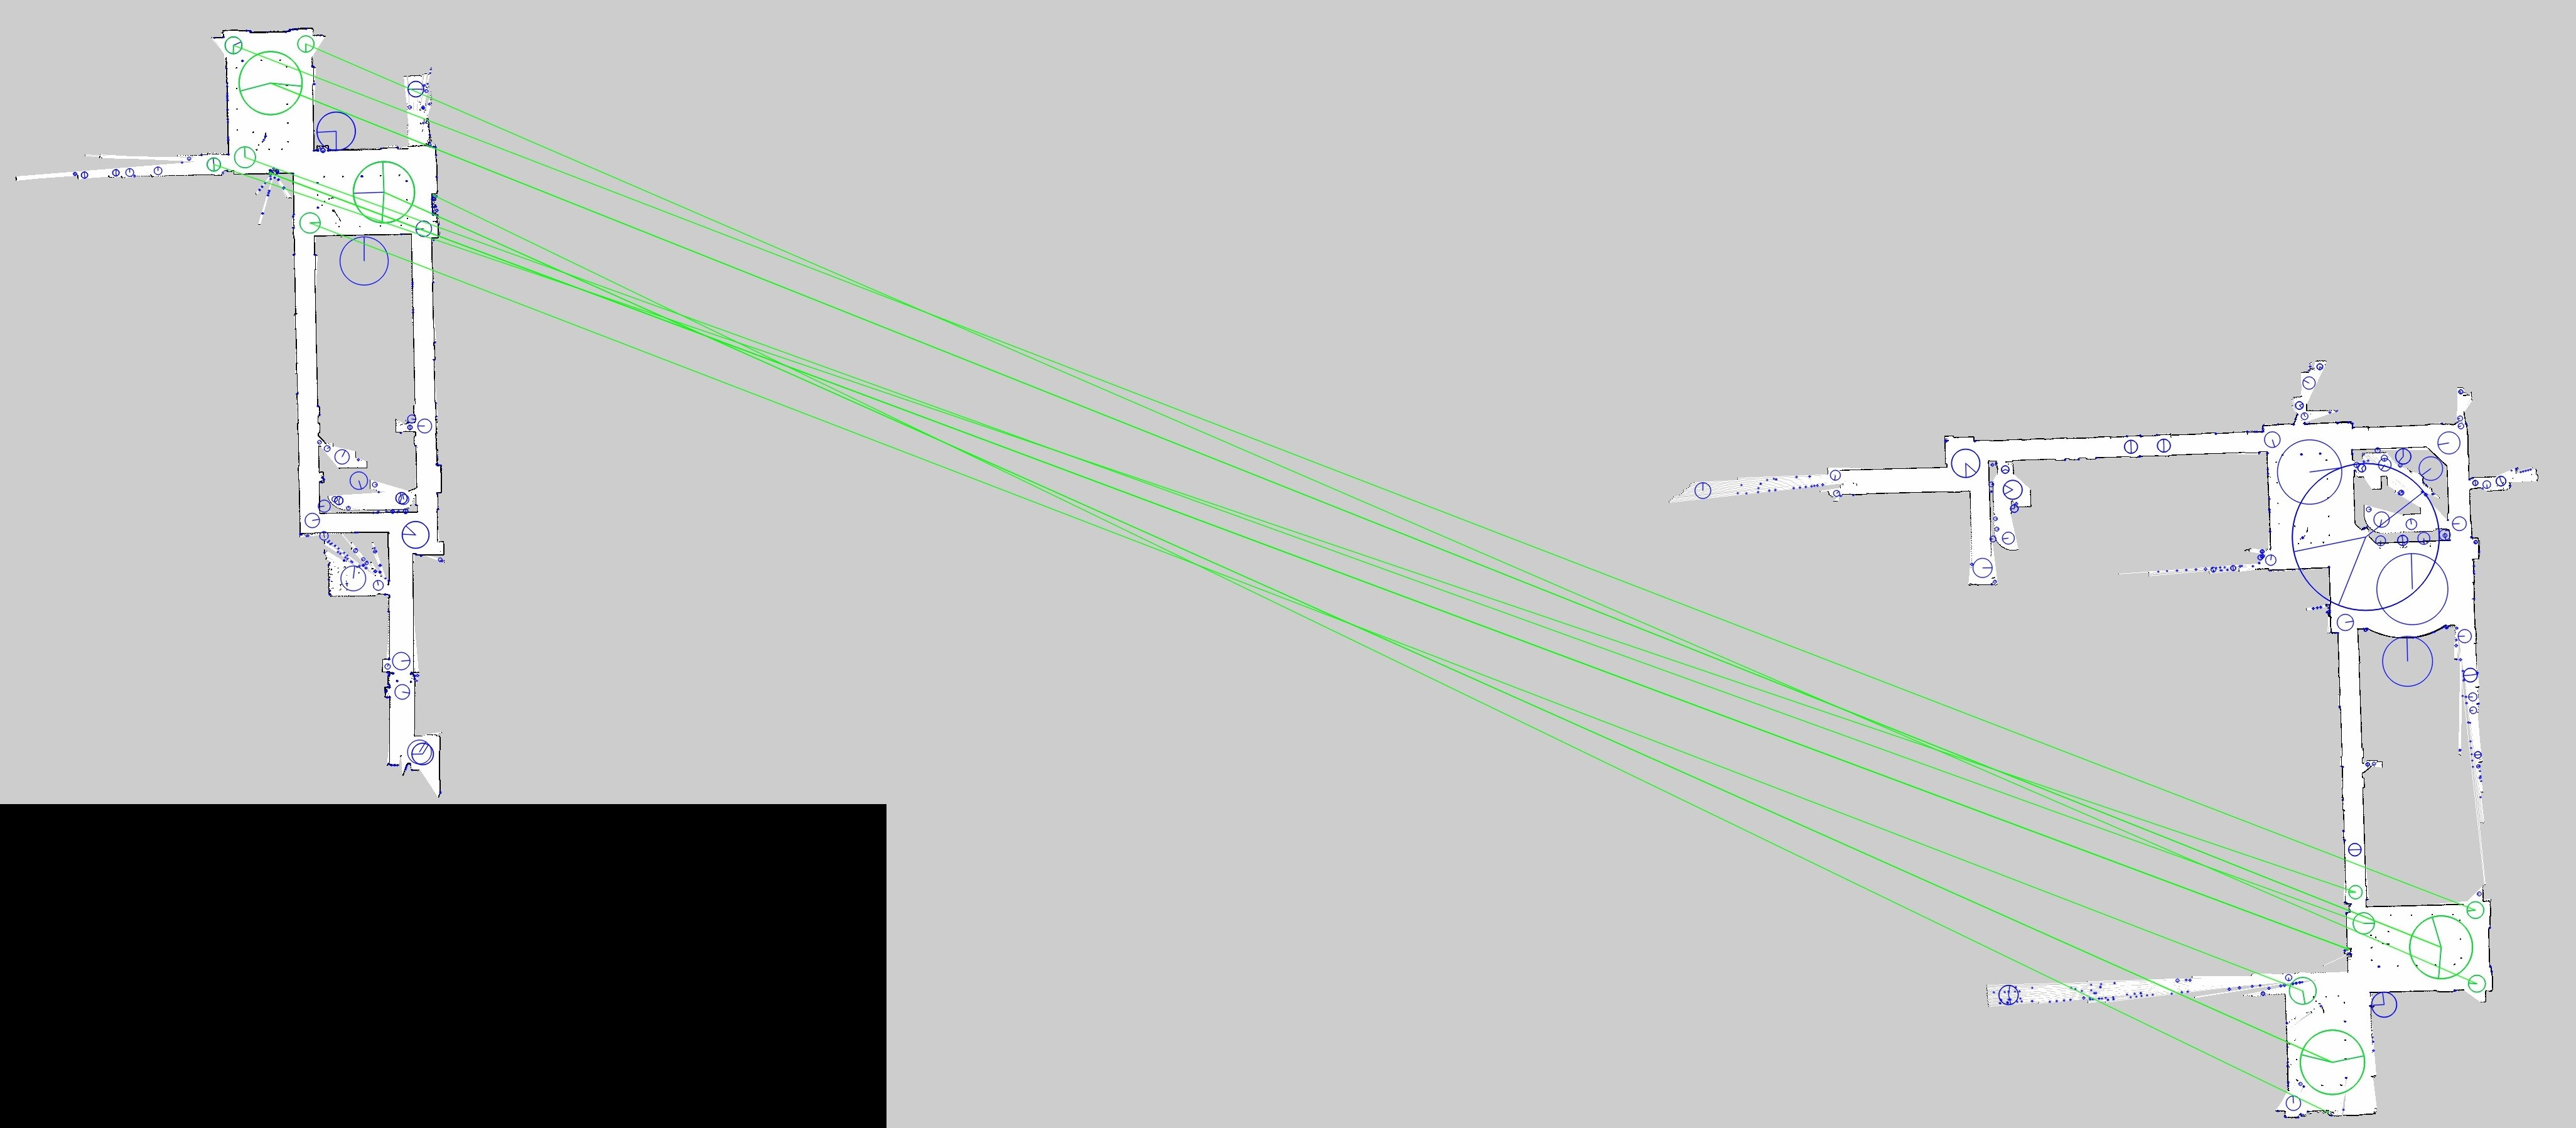
\includegraphics[width=1\textwidth]{figs/real_world_results/a/matchesPartialMap1Map3.jpg}
    \caption{The matched features between partial map\_1 and map\_3 are presented in this figure. The features highlighted in green, are the features that have been matched between the two maps}
    \label{fig:real3matches2}
\end{figure} 
%....................................................

%....................................................
\begin{figure}[H]
    \centering
    \includegraphics[width=1\textwidth]{figs/real_world_results/a/matchesPartialMap1Map4.jpg}
    \caption{The matched features between partial map\_1 and map\_4 are presented in this figure. The features highlighted in green, are the features that have been matched between the two maps}
    \label{fig:real3matches3}
\end{figure} 
%....................................................


%....................................................
\begin{table}[H]
\centering
\caption{This table presents the results from the alignment and merging operation. Since the partial maps are merged relatively to map\_1 the results are relative to map\_1, which  has a resolution of 0.05 m/cell.}
\begin{tabular}{ | m{1.2cm} | m{2cm} | m{2cm} | m{2.2cm} | m{1.7cm} | m{1.2cm} | m{2.2cm} |} 
\hline
\textbf{Map} & \textbf{Resolution (m/cell)} & \textbf{New resolution (m/cell)} & \textbf{Angle of rotation (\degree)} & \textbf{Good matches}& \textbf{Match ratio} & \textbf{Percentage overlap}\\ 
\hline
\hline
Partial map\_2  & 0.05 & 0.05014256 & 41.6208106 & 242 & 0.49 & 51.60\\ 
\hline
Partial map\_3  & 0.05 & 0.05007269 & -89.0525206 & 201 & 0.55 & 23.71\\ 
\hline
Partial map\_4  & 0.1  & 0.05011043 & 5.67170818 & 115 & 0.91 & 39.37\\ 
\hline
\end{tabular}
\label{table:real3}
\end{table}
%....................................................


%====================================================
\subsubsection{Summary}
%----------------------------------------------------

Overall the real-world experiments show that the solution can handle real-world scenarios. Hence partial maps of varying resolution, translation and orientation; can be aligned and merged. Furthermore, this section shows that the match ratio and percentage overlap are not directly proportional, as observed before. The next section will further test the solutions ability to handle partial maps generated from publicly available data.


%====================================================
\section{MIT Stata Center experiments}
\label{sec:ch4.section2}
%----------------------------------------------------

The solution is further tested using a publicly available data-set, in this section. 

%====================================================
\subsection{Environment setup}
\label{sec:ch4.subsecMIT}
%----------------------------------------------------

The data-set is presented in Section\ref{sec:ch4.subsecMIT}, and this data is accessed using the capability of ROS \(rosbag\). The Hokuyo UTM-30LX Laser scan data is used as an input to \(Hector\_Mapping\) to generate the partial maps at varying resolutions.
The Massachusetts Institute of Technology (MIT) Stata Center Data Set is a vast scale data-set collected between 2011 and 2013. The academic building is a size of 67,000 $m^2$ and contains 10 storeys \cite{doi:10.1177/0278364913509035}. The collected data-set comprises of over 2.3TB, 38 hours and 42 km of sensor data, and can be accessed on the university website\footnote{https://projects.csail.mit.edu/stata/}. This set is of particular interest to robotics and computer vision researchers; due to the following rich sensor data:

\begin{center}
\begin{tabular}{ | m{5cm} | m{2cm}| } 
\hline
Sensor & Frequency \\ 
\hline
\hline
 Hokuyo UTM-30LX Laser  & 40 Hz\\ 
\hline
Wheel Odometry [Raw] & 44 Hz \\ 
\hline
Wheel Odometry [Integrated] & 25 Hz \\ 
\hline
Microstrain 3DM-GX2 IMU	& 10 Hz \\
\hline
Willow Garage Stereo & 30 Hz \\
\hline
Microsoft Kinect & 30 Hz \\
\hline
\end{tabular}
\end{center}

The data were recorded using \(rosbag\) on ROS; therefore, it can be played back and used to produce partial maps in this thesis. To test the solution, the \(hector\_mapping\) ROS node is run using Hokuyo UTM-30LX Laser sensor data to produced partial maps at varying resolution.

%====================================================
\subsection{Results and discussion}
%----------------------------------------------------

In this section, results from the MIT Stata Center data are presented.

%==================================================== 
\subsubsection{Experiment one} %----------------------------------------------------


The initial MIT experiment is Figure \ref{fig:mit1} considers partial maps of the same resolution of 0.1 m/cell. Figures \ref{fig:mit11}, \ref{fig:mit12} and \ref{fig:mit13} presented the partial maps before the alignment and merging operation. Figure \ref{fig:mit14} presents the global map after alignment and merging of the three partial maps. The new resolution of partial\_map\_2 and partial\_map\_3 are within 1\% of partial\_map\_1's resolution (shown in Table \ref{tab:mit1}), therefore validating the success of the alignment operation.



%....................................................
\begin{figure}[H]
%----------------------------------------------------
\begin{subfigure}{0.5\textwidth}
%----------------------------------------------------
\includegraphics[width=0.9\linewidth, height=5cm]{figs/mit_results/a/partial_map_1.jpg}
%----------------------------------------------------
\caption{Partial map\_1 resolution of 0.1 m/cell}
%----------------------------------------------------
\label{fig:mit11}
%----------------------------------------------------
\end{subfigure}
%----------------------------------------------------
\begin{subfigure}{0.5\textwidth}
%----------------------------------------------------
\includegraphics[width=0.9\linewidth, height=5cm]{figs/mit_results/a/partial_map_2.jpg} 
%----------------------------------------------------
\caption{Partial map\_2 with resolution of 0.1 m/cell}
%----------------------------------------------------
\label{fig:mit12}
\end{subfigure}
\begin{subfigure}{0.5\textwidth}
\includegraphics[width=0.9\linewidth, height=5cm]{figs/mit_results/a/partial_map_3.jpg} 
\caption{Partial map\_3 with resolution of 0.1 m/cell}
\label{fig:mit13}
\end{subfigure}
\begin{subfigure}{0.5\textwidth}
\centering
\includegraphics[width=0.9\linewidth, height=5cm]{figs/mit_results/a/final_map.jpg} 
\caption{Final map with resolution of 0.1 m/cell}
\label{fig:mit14}
\end{subfigure}
\caption{Three partial maps and a global map are presented. The partial maps are generated from publicly available data.  Since the maps are aligned relative to map1, the resultant global map will have the same resolution as partial map\_1}
\label{fig:mit1}
\end{figure}
%....................................................


Figure \ref{fig:mit1matches1} shows the feature matches between partial map\_1 and map\_2, with a match ratio of 0.55 in an overlap region of 11.08\% (see Table \ref{tab:mit1}). The overlap percentage of 11.08\% is the lowest value observed so far. This percentage overlap suggests that the map merging algorithms performance is dependent on the match ratio rather than the percentage of overlap. Figure \ref{fig:mit1matches2} shows the feature matches between partial map\_1 and map\_3, with a match ratio of 0.70 in an overlap region of 29.03\% (see Table \ref{tab:mit1}).


%....................................................
\begin{figure}[H]
    \centering
    \includegraphics[width=1\textwidth]{figs/mit_results/a/matchesPartialMap1Map2.jpg}
    \caption{The matched features between partial map1 and map2 are presented in this figure. The features highlighted in green, are the features that have been matched between the two maps}
    \label{fig:mit1matches1}
\end{figure} 
%....................................................

%....................................................
\begin{figure}[H]
    \centering
    \includegraphics[width=1\textwidth]{figs/mit_results/a/matchesPartialMap1Map3.jpg}
    \caption{The matched features between partial map\_1 and map\_3 are presented in this figure. The features highlighted in green, are the features that have been matched between the two maps}
    \label{fig:mit1matches2}
\end{figure} 
%....................................................

%....................................................
\begin{table}[H]
\centering
\caption{This table presents the results from the alignment and merging operation. Since the partial maps are merged relatively to map\_1 the results are relative to map\_1, which  has a resolution of 0.1 m/cell.}
\begin{tabular}{ | m{1.4cm} | m{2.2cm} | m{2.2cm} | m{2.4cm} | m{1.7cm} | m{1.4cm} | m{2.4cm} | }
\hline
\textbf{Map} & \textbf{Resolution (m/cell)} & \textbf{New resolution (m/cell)} & \textbf{Angle of rotation (\degree)} & \textbf{Good Matches} & \textbf{Match ratio} & \textbf{Percentage overlap}\\ 
\hline
\hline
Partial map\_2  & 0.1  & 0.09972303 & -174.1462356 & 92 & 0.55 & 11.08\\ 
\hline
Partial map\_3  & 0.1  & 0.10033173 & -14.49865513 & 135 & 0.70 & 29.03\\ 
\hline
\end{tabular}
\label{tab:mit1}
\end{table}
%....................................................



%==================================================== 
\subsubsection{Experiment two} %----------------------------------------------------

Figures \ref{fig:mit21}, \ref{fig:mit22} and \ref{fig:mit23} presented the partial maps before the alignment and merging operation, with resolutions of 0.1 m/cell, 0.1 m/cell and 0.11 m/cell respectively . Figure \ref{fig:mit24} presents the global map after alignment and merging of the three partial maps. The new resolution of partial\_map\_2 and partial\_map\_3 are within 1\% of partial\_map\_1's resolution (shown in Table \ref{tab:mit2}), therefore validating the success of the alignment operation.

%....................................................
\begin{figure}[H]
\begin{subfigure}{0.5\textwidth}
\includegraphics[width=0.9\linewidth, height=5cm]{figs/mit_results/b/partial_map_1.jpg} 
\caption{Partial map\_1 with resolution of 0.1 m/cell}
\label{fig:mit21}
\end{subfigure}
\begin{subfigure}{0.5\textwidth}
\includegraphics[width=0.9\linewidth, height=5cm]{figs/mit_results/b/partial_map_2.jpg} 
\caption{Partial map\_2 with resolution of 0.1 m/cell}
\label{fig:mit22}
\end{subfigure}
\begin{subfigure}{0.5\textwidth}
\includegraphics[width=0.9\linewidth, height=5cm]{figs/mit_results/b/partial_map_3.jpg} 
\caption{Partial map\_3 resolution of 0.11 m/cell}
\label{fig:mit23}
\end{subfigure}
\begin{subfigure}{0.5\textwidth}
\centering
\includegraphics[width=0.9\linewidth, height=5cm]{figs/mit_results/b/final_map.jpg} 
\caption{Final map with resolution of 0.1 m/cell}
\label{fig:mit24}
\end{subfigure}
\caption{Three partial maps and a global map are presented. The partial  maps are generated from publicly available data. Since the maps are aligned relative to map\_1, the resultant global map will have the same resolution as partial map\_1}
\label{fig:mit2}
\end{figure}
%....................................................


Figure \ref{fig:mit2matches1} shows the feature matches between partial map\_1 and map\_2, with a match ratio of 0.70 in an overlap region of 39.63\% (see Table \ref{tab:mit2}). Figure \ref{fig:mit2matches2} shows the feature matches between partial map\_1 and map\_3, with a match ratio of 0.85 in an overlap region of 13.59\% (see Table \ref{tab:mit2}). Here we observe another low percentage overlap of 13.59\% with a high match ratio of 0.85.


%....................................................
\begin{figure}[H]
    \centering
    \includegraphics[width=1\textwidth]{figs/mit_results/b/matchesPartialMap1Map2.jpg}
    \caption{The matched features between partial map\_1 and map\_2 are presented in this figure. The features highlighted in green, are the features that have been matched between the two maps}
    \label{fig:mit2matches1}
\end{figure} 
%....................................................

%....................................................
\begin{figure}[H]
    \centering
    \includegraphics[width=1\textwidth]{figs/mit_results/b/matchesPartialMap1Map3.jpg}
    \caption{The matched features between partial map\_1 and map\_3 are presented in this figure. The features highlighted in green, are the features that have been matched between the two maps}
    \label{fig:mit2matches2}
\end{figure} 
%....................................................

%....................................................
\begin{table}[H]
\centering
\caption{This table presents the results from the alignment and merging operation. Since the partial maps are merged relatively to map1 the results are relative to map1 which has a resolution of 0.1 m/cell.}
\begin{tabular}{ | m{1.4cm} | m{2.2cm} | m{2.2cm} | m{2.4cm} | m{1.7cm} | m{1.4cm} | m{2.4cm} | }
\hline
\textbf{Map} & \textbf{Resolution (m/cell)} & \textbf{New resolution (m/cell)} & \textbf{Angle of rotation (\degree)} & \textbf{Good matches} & \textbf{Match ratio} & \textbf{Percentage overlap}\\ 
\hline
\hline
Partial map\_2  & 0.1  & 0.100164329 & -0.010020086 & 133 & 0.70 & 39.63\\ 
\hline
Partial map\_3  & 0.11  & 0.105664826 & 139.9271825 & 94 & 0.85 & 13.59\\ 
\hline
\end{tabular}
\label{tab:mit2}
\end{table}
%....................................................

%====================================================
\subsubsection{Summary}
%----------------------------------------------------

This section shows that the solution can align and merge partial maps from other real-world data-sets produced by other authors. This result benchmarks the solution with other similar approaches. The results further demonstrate the algorithm ability to merge maps with a percentage overlap as low as 11.08\%.



%====================================================
\section{Summary}
\label{sec:ch4.section4}
%----------------------------------------------------

This chapter has tested the solution presented in Chapter \ref{ch:implementation}. We found its performance acceptable, dealing with simulated and real-world scenarios. The technique can successfully align and merge maps gathered from multiple robots, with partial maps of different orientation, translation and resolution.

In the next chapter, we will reflect upon the work done in this dissertation and analyse the results in light of the requirements in Chapter \ref{ch:ch1}. We will also explore the possible further work that can be done to expand on the work.



%****************************************************
% END
%****************************************************
